\documentclass[11pt, oneside]{report}   	% use "amsart" instead of "article" for AMSLaTeX format
%notitlepage puts the abstracts in different languages on the same page
\usepackage{geometry}                		% See geometry.pdf to learn the layout options. There are lots.
\geometry{letterpaper}                   		% ... or a4paper or a5paper or ... 
%\geometry{landscape}                		% Activate for for rotated page geometry
%\usepackage[parfill]{parskip}    		% Activate to begin paragraphs with an empty line rather than an indent
\usepackage{graphicx}				% Use pdf, png, jpg, or eps§ with pdflatex; use eps in DVI mode
								% TeX will automatically convert eps --> pdf in pdflatex	
%\usepackage[utf8]{inputenc}
\usepackage[T1]{fontenc}	
\usepackage{amssymb}
\usepackage{amsmath}
\usepackage{amsthm}
\usepackage{enumitem}
\usepackage{mathrsfs}
%\usepackage{bbold}
\usepackage{hyperref}
%\usepackage{cleveref}
%\usepackage{stmaryrd}
\usepackage{slashed}
%\usepackage{color}
%\usepackage[ngerman,french,english]{babel}

\graphicspath{{images/}}

%\usepackage[numbers,sort]{natbib}


\newcommand{\cref}[1]{Eq.(\ref{#1})}
\newcommand{\ie}{\textit{i.e., }}
\newcommand{\eg}{\textit{e.g. }}
\newcommand{\wrt}{w.r.t. }
\newcommand{\rhs}{r.h.s. }
\newcommand{\lhs}{l.h.s. }
\newcommand{\eval}[1]{\bigg\rvert_{#1}}
\newcommand{\dd}{\textrm{d}}
%\newcommand{\de}{\textrm{e}}
\newcommand{\im}{\mathrm{Im}}
\newcommand{\ran}{\mathrm{Ran}}
\newcommand{\rank}{\mathrm{Rank}}
\newcommand{\dom}{\mathrm{Dom}}
\newcommand{\en}{\mathrm{End}}
\newcommand{\tr}{\mathrm{Tr}}
\newcommand{\grad}{\mathrm{grad}}
\newcommand{\res}{\mathrm{Res}}

%equation with split DOESN'T WORK...
%\def\sequation#1#2{\begin{equation}\label{#2}\begin{split}{#1} \end{split} \end{equation} }
%\def\sequationstr#1{\begin{equation*}\begin{split}{#1} \end{split} \end{equation*}}

\newtheorem{theorem}{Theorem}
\newtheorem{lemma}{Lemma}
\newtheorem{proposition}{Proposition}
\newtheorem{definition}{Definition}
\theoremstyle{remark}
\newtheorem{remark}{Remark}

\title{M2 internship}
\author{En-hung CHAO}
%\date{}							% Activate to display a given date or no date
\usepackage[colorinlistoftodos]{todonotes}

\begin{document}

%\maketitle
%title page

\begin{titlepage}

\newcommand{\HRule}{\rule{\linewidth}{0.5mm}} % Defines a new command for the horizontal lines, change thickness here

\center % Center everything on the page
 
%----------------------------------------------------------------------------------------
%	HEADING SECTIONS
%----------------------------------------------------------------------------------------

\textsc{\LARGE {\'E}cole Normale Sup{\'e}rieure  }\\[0.3cm] % Name of your university/college
%\textsc{\LARGE INSTITUTE OF TECHNOLOGY  }\\[0.3cm]
%\textsc{\Large JALANDHAR-144011, PUNJAB(INDIA) }\\[0.3cm]
\textsc{\Large Research internship of the M2 ICFP program}\\[0.5cm] % Major heading such as course name
 % Minor heading such as course title

%----------------------------------------------------------------------------------------
%	TITLE SECTION
%----------------------------------------------------------------------------------------

\HRule \\[0.4cm]
{ \huge \bfseries Unitarity method in one-loop QCD amplitudes}\\[0.03cm] % Title of your document
\HRule \\[1.5cm]

 
%----------------------------------------------------------------------------------------
%	AUTHOR SECTION
%----------------------------------------------------------------------------------------

\begin{minipage}{0.4\textwidth}
\begin{flushleft} \large
\emph{Author:}\\
En-Hung CHAO  \\Master 2 ICFP \\theoretical physics option \\ {\'E}cole Normale Sup{\'e}rieure (Paris, France)% Your name
~
\end{flushleft}
\end{minipage}
\begin{minipage}{0.4\textwidth}
\begin{flushright} \large
\emph{Supervised by:} \\
Dr. David Kosower \\Institut de Physique Th{\'e}orique \\Commissariat {\`a} l'{\'E}nergie Atomique (Saclay, France) % Supervisor's Name 
\end{flushright}
\end{minipage}\\[1cm]

% If you don't want a supervisor, uncomment the two lines below and remove the section above
%\Large \emph{Author:}\\
%John \textsc{Smith}\\[3cm] % Your name

%----------------------------------------------------------------------------------------
%	DATE SECTION
%----------------------------------------------------------------------------------------

{\large April 3rd - June 29th, 2018 \\Research internship at \\ Institut de Physique Th{\'e}orique}, CEA Saclay\\[1cm] % Date, change the \today to a set date if you want to be precise

%----------------------------------------------------------------------------------------
%	LOGO SECTION
%----------------------------------------------------------------------------------------

\begin{minipage}{0.4\textwidth}
\begin{flushleft} \large
\centering

\includegraphics[scale=0.4]{ens_logo}\\[1cm] % Include a department/university logo - this will require the graphicx package
  
\end{flushleft}
%\end{minipage}\\[1cm]
%\begin{minipage}{0.4\textwidth}
\begin{flushright} \large
\centering

\includegraphics[scale=0.1]{cea_logo}\\[1cm] % Include a department/university logo - this will require the graphicx package
  
\end{flushright}
\end{minipage}\\[1cm]
%----------------------------------------------------------------------------------------

\vfill % Fill the rest of the page with whitespace

\end{titlepage}

%%%%%%%%%%%%%%%%%%%%%%%%%%%%%%%%%%%%%%%%%%%%%%%%%%%%%%%%%%%%%%%%%%%%%
\iffalse
%--------------------------------------
\section*{Abstract}
This work consists of two parts.
In the first one, we investigate the vacuum polarization in 1+1 dimension in the presence of a Kondo-type potential.
We apply the renormalization by point-splitting \wrt the  Hadamard parametrix to evaluate the vacuum charge density and the vacuum stress-energy tensor.
In the second part, we study the Wentzell boundary condition for massless fermions.
After proving the well-posedness of dynamical problems and the property of causal propagation under this boundary condition, we discuss the vacuum polarization and the vacuum stress-energy tensor in using the same renormalization technique as in the first part.

\section*{Résumé}
Ce travail consiste en deux parties. 
Dans la première partie, nous nous intéressons à la polarisation du vide en dimension 1+1 en présence d'un poteniel singulier dit de "type Kondo".
Nous appliquons la renormalisation par point-splitting par rapport au parametrix d'Hadamard afin d'évaluer la densité de charge du vide et le tenseur d'énergie-impulsion du vide.
Dans la seconde partie, nous étudions la condition aux limites de Wentzell pour les fermions de masse nulle.
Après avoir prouvé que les problèmes dynamiques sont bien posés sous cette condition aux limites généralisée et la propriété de propagation causale,
nous discutons de la polarisation du vide ainsi que le tenseur d'énergie-impulsion du vide en utilisant la même technique de renormalisation introduite dans la première partie.

\newpage
%-----------------------------------------
%acknowledgement
\section*{Acknowledgements}
I am very grateful to my supervisor, Dr. Jochen Zahn, for his constructive and patient mentoring during the entire period of the internship, and also for his suggestions and reviews during the writing of this report afterwards.
The hospitality of Elementary Particle Theory Group of Insitute of Theoretical Physics of University of Leipzig (Germany), directed by Prof. Stefan Hollands, is greatly appreciated.
Besides, I would also like to thank Onirban Islam (University of Leipzig), Mojtaba Taslimitehrani (University of Leipzig) and Alexandre Efremov (École Polytechnique) for useful discussions and recommendations for literatures. 
\fi
%%%%%%%%%%%%%%%%%%%%%%%%%%%%%%%%%%%%%%%%%%%%%%%%%%%%%%%%%%%%%%%%%%%%%%%%%


%\tableofcontents
\section{Introduction}
Recent progress in collider technology allows experiments at the Large Hadron Collider (LHC) to be conducted at the TeV scale.
The detection of new physics at the scale of electroweak symmetry breaking becomes of great interest. 
Quantum corrections at higher order become crucial for studying physically relevant signals. 
Especially, next-to-leading (NLO) corrections in quantum chromodynamics (QCD) play an important role. 
For example, differential cross section computations require processes beyond tree-level, such as real gluon emissions, formation of jets and virtual one-loop corrections.
However, traditional diagrammatic amplitude computations become highly complicated in gauge theories at loop-level.
One-loop results in QCD were only known up to five external legs before the early nineties~\cite{Bern:1994zx}. 
During the past twenty years, many breakthroughs in amplitude computations have been made at both tree-level and one-loop.
The main propose of this internship report is to give an overview of how to use on-shell recursion and generalized unitarity to get tree-level and one-loop amplitudes in an efficient way. 
The actual threshold of amplitude computation is at the next-to-next-to-leading order (NNLO), which these techniques are being generalized to.
\\\\
Tree-level amplitude computations are more simple since they do not require any potentially divergent loop integral.
Nevertheless, in a gauge theory, the complexity of the calculation still increases phenomenally when the number of external legs increases.
Due to Britto, Cachazo, Feng and later Witten~\cite{BRITTO2005499, PhysRevLett.94.181602}
tree-level amplitudes can be computed recursively in the number of external legs.
The BCFW recursion, or known as on-shell recursion, makes use of complex analysis to relate a higher-point amplitude to lower-point ones by studying the poles of an analytic function contructed out of an n-point amplitude.
This method does not require the knowledge of any individual Feynman diagram, but only needs the behavior of the analytic function when certain combinations of external momenta go "on-shell". 
In a massless gauge theory, the recursion relation of color-ordered amplitudes can be written in a compact way using the spinor-helicity formalism.
In particular, we can recover the Taylor-Parke formula for maximally-helicty-violation (MHV) amplitudes (\ie only two particles have a helicity different from the others.) from on-shell recursion.
\\\\
In the early nineties, Bern, Dixon, Dunbar and Kosower~\cite{Bern:1994zx} proposed a method based on the Cutkosky rules~\cite{doi:10.1063/1.1703676}, or known as generalized unitarity, which became later an important basis for one-loop amplitude computation tools.
It is known that an $m$-point integral can be reduced into integrals of lower degree (\eg by a Passarino-Veltman reduction~\cite{PASSARINO1979151}).
Although in the presence of massless propagators, one might use the dimension regularization scheme to control the infrared divergences and work in $D = 4-2\epsilon$ dimension, it can be proven that loop integrals can be written in a basis composed of bubble, triangle and box integrals (\ie two-, three- and four-point integrals), called the master integrals, up to the order of $\mathcal{O}(\epsilon^0)$ (see \eg~\cite{Gluza:2010ws} for a review).
Generalized unitarity consists in "cutting" one or several loop propagators in the same time by putting them on-shell.
Mathematically, this corresponds to the branch cut at the channel where the cut is performed. 
To be more precise, since the master integrals contain logarithms and dilogarithms, this equals to the imaginary part of the final loop amplitude when a certain kinematic invariant changes sign.
After doing so, an one-loop amplitude becomes a product of several tree-level amplitudes integrated over the phase-space of all possible intermediate species.
In a theory with supersymmetry, this task becomes even more simple thanks to the super-symmetry Ward identities which relate one species to another.
An even particular case, where the generalized unitarity was first tested~\cite{Bern:1994zx}, is the N=4 super-Yang-Mills (SYM) theory, whose one-loop amplitudes involve uniquely scalar box integrals. 
\\\\
During the last decade, methods to extract coefficients of master integrals were developped. 
A procedure to extract the box coefficients using quadruple cuts, \ie with four internal propagators put on-shell, was proposed by Britto, Cachazo and Feng~\cite{Britto:2004nc}. 
This procedure was originally formulated in four-dimension, where a quadruple cut leads to four delta functions, which makes the integral over the phase-space trivial to compute. 
However, to make this idea clear, complex momenta~\cite{PhysRevD.75.025028} have to be used for the delta functions.
By a wise choice of parametrization, Forde shows~\cite{Forde:2007mi} an efficient way to extract bubble and triangle coefficients using triple cuts in $D=4$.
Contrary to the quadruple cut case, there will still be remaining degrees of freedom for two-particle and triple cuts. 
Forde's parametrization reduces the number relevant polynomial terms in these degrees of freedom which should be taken into account during the extraction. 
Note that not all the theories are cut-constructible, \ie whose amplitudes can be determined totally by cuts~\cite{Bern:1994cg}. 
A further ambiguity is the rational term, \ie an additional polynomial in kinetic invariant in the expression of an amplitude. 
Rational terms do not have branch cut when kinetic invariants change regime, thus they will result in vanishing contributions in cut amplitudes.
In a cut-constuctible theory, the issue of rational term still exists due to the dimensional regularization scheme. 
Based on previous works in four-dimensions, Badger shows how rational terms can be determined~\cite{Badger:2008cm}
\\\\
All these tools described above enable us to compute amplitudes for all helicities at one-loop.
In this report, we will review them in the following order.
We start with a brief introduction on the spinor-helicity formalism, general facts in color-ordered amplitudes and on-shell recursion.
An explicit computation using the on-shell recursion will be done for the five-point MHV tree-level gluon amplitude. 
Then, we sketch the idea of the Cutkosky rules and verify the statement with the examples of cuts in the s-channel of the one-mass triangle and two-mass-easy box, with massless internal propagators.
Later on, we concentrate on the generalized unitarity applied to one-loop in N=4 SYM.
We will review the "only-box" property of one-loop amplitudes in N=4 SYM by following~\cite{Bern:1994zx} and the different coefficient extraction techniques in four-dimension. 
At the end, we will compute the five-point one-loop MHV gluon amplitude in N=4 SYM.












%\subsection*{$A_5^{\mathrm{1-loop}}[1^-2^-3^+4^+5^+]$ in $\mathcal{N}=4$ super Yang-Mills}\label{sect-a5mhv}
Let us see how to use quadruple cuts to extract box coefficients by computing the all-gluon MHV amplitude $A_5^{\mathrm{1-loop}}[1^-2^-3^+4^+5^+]$ in $\mathcal{N}=4$ super Yang-Mills. 
There are five possible configurations for the external momenta under a quadruple cut.
Each of the configurations corresponds to a one-mass box integral.
Among the four tree-level amplitudes that we obtain from a quadruple cut~\cref{box_coeff}, there is a four-point amplitude and three three-point ones.
As already noted in the original quadruple cut paper~\cite{Britto:2004nc}, massless legs in quadruple cut would lead to inconsistent results if we choose loop-momentun to be real\footnote{This was handled in~\cite{Britto:2004nc} by working in the signature $(--++)$.}. 
However, in the contour integral scheme with complex loop momentum that we mentioned earlier, this problem is not present.
\\\\
Next, let us consider all the possible helicity configuration on the cuts.
To start, we may take all the internal particles to be gluons. 
Then, we relate the all-gluon tree-level amplitudes to other amplitudes with different species by~\cref{super_wi}. 
By the discussion given in section~\ref{sect-spinor}, we have to have exactly two particles of the same helicity in order to get non-vanishing contribution from three- and four-point tree-level amplitudes~\cref{a3mhv} and~\cref{parke-taylor}.
Up to this step, we have already eliminated a bunch of helicity configurations
\\\\
Finally, the on-shell condition of the internal propagtors may in certain case impose further relationships to the external momenta than just the momentum conservation.
These cases should also be discarded because they violate our requirement of non-collinearity of the external momenta. 
%\color{red}perhaps describe more with a graph.\color{black}
At the end of the day, there are only five possible solutions to the all-gluon configuration (figure~\ref{fig-a5mhv}).
We give the detailed computation hereunder.
\begin{figure}
  \centering
  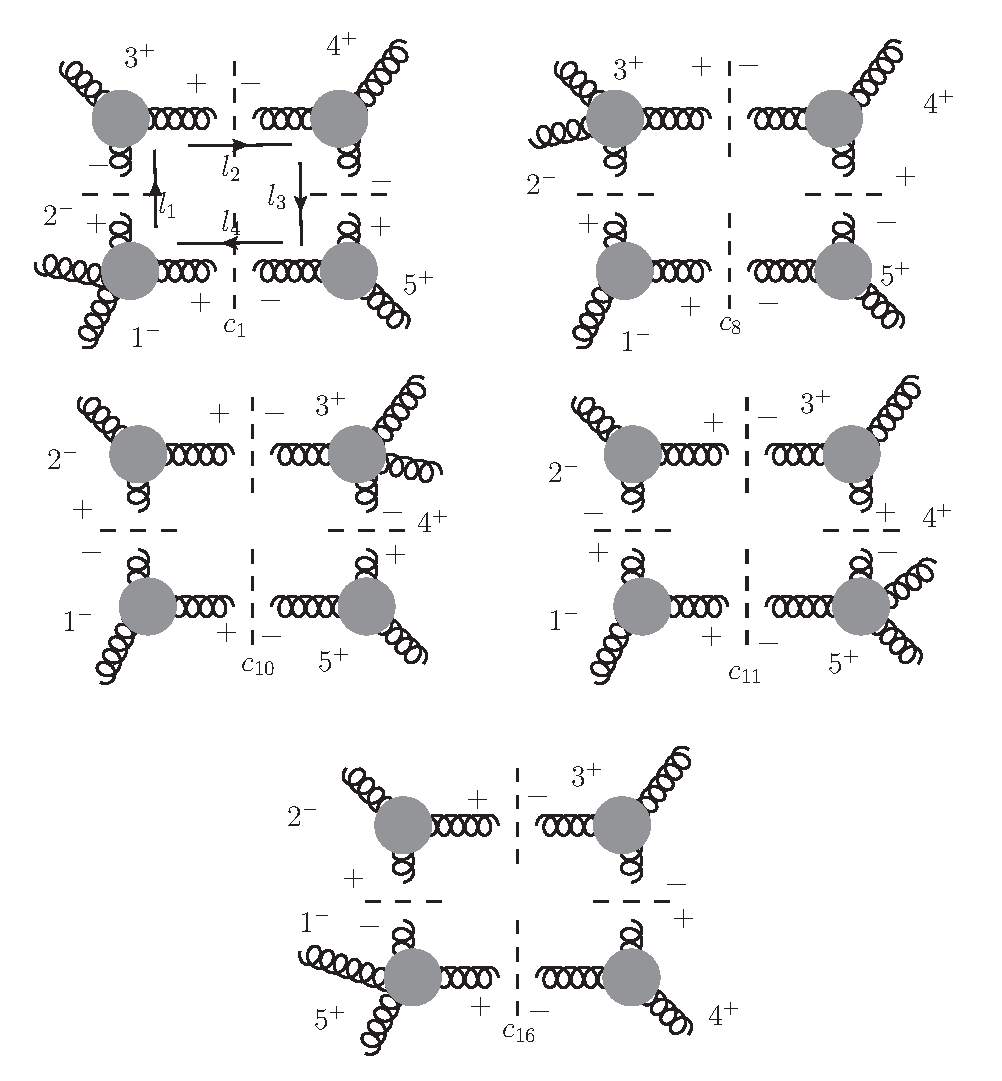
\includegraphics[width=0.8\linewidth]{A5mhv.eps}
  \caption{The only non-vanishing contributions for $A_5^{\mathrm{1-loop}}[1^-2^-3^+4^+5^+]$ in $\mathcal{N}=4$ super Yang-Mills. The momenta in the loop are enumerated in the same way as the top-left one.}
  \label{fig-a5mhv}
\end{figure}
\paragraph{Configuration $c_1$}
The special three-particle kinematics tells us that either the square spinor product or the angle one of any two on-shell spinor linked to a trivalent vertex vanishes.
By considering the trivalent vertices appearing in this configuration, the only possible solution for the internal momenta in terms of spinors should satisfy
\begin{equation}
|l_1\rangle = \alpha |5\rangle \quad,\quad
|l_2\rangle = \delta |3\rangle \quad,\quad
|l_3\rangle = \gamma |l_3\rangle\quad,\quad
|l_3] = \eta|4]\quad,\quad
|l_4] = \beta |4]
\end{equation}
Hence, the coefficient determined by~\cref{box_coeff} is
\begin{equation}\label{coef_c_1}
\begin{split}
c_1 = &
\frac{1}{2}\frac{\langle 12 \rangle^4}{\langle 1 2 \rangle \langle 2 l_2\rangle \langle l_2 l_1 \rangle\langle l_1 1 \rangle}
\frac{[3l_3]^3}{[l_3 l_2][l_2 3]}
\frac{\langle l_3 l_4 \rangle^{3}}{\langle l_4 4 \rangle \langle 4 l_3\rangle}
\frac{[l_4 5 ]^3}{[5l_1][l_1 l_4]}
\\
= & 
\frac{1}{2}\frac{\langle 12 \rangle^3}{\langle 2 l_2 \rangle\langle l_2 l_1 \rangle\langle l_1 1\rangle}
\frac{[34]^2\langle l_4 4\rangle}{[l_3 l_2][l_2 3]\langle 4 l_3\rangle}
\frac{[l_4 5]^2}{[5l_1 ][l_1 l_4]}
[3 l_3]\langle l_3 l_4 \rangle [l_4 5]
\\
= &
\frac{1}{2}
\frac{\langle 12 \rangle^3[34]^2[45]}{\langle 15 \rangle\langle2|\slashed{K}_{3}|4]}
\\
= &
\frac{1}{2}\frac{\langle 12 \rangle^4 s_{34}s_{45}}{\langle 12 \rangle\langle 23 \rangle \langle 34\rangle \langle 45\rangle \langle 51\rangle}
\\
= &
\frac{1}{2}s_{34}s_{45}A_5^{\textrm{MHV-tree}}[12345]
\end{split}
\end{equation}
We list here the results for the other contributions. 
The explicit computations are given in Appendix~\ref{appendix-a5mhv}\footnote{
In fact, the knowledge of $c_1$ suffices to obtain the full amplitude.
In a supersymmetric theory, we can derive any amplitude from a super-amplitude using the superspace formulation (see \eg ref~\cite{Elvang:2013cua} for an introduction). 
In an $\mathcal{N} = 4$ theory, the relationship between an $n$-point MHV amplitude and the relevant super-amplitude $\mathcal{A}_n$ at all level is uniquely determined by the knowledge at tree-level and is given by~\cite{Elvang:2010xn} 
\begin{equation}
\mathcal{A}_n^{\mathrm{MHV}} = \delta^{8}(\tilde{Q})\frac{1}{\langle n-1, n\rangle^4}A_n^{\mathrm{tree}}[+,+,\ldots,+,-,-]
\end{equation}
where $\tilde{Q}$ represents the set of supersymmetry generators.
As one can notice from this expression, the term on the right hand side should be cyclic. 
As a result, to determine the five-point MHV amplitude, it suffices to take~\cref{coef_c_1}, multiply it with the box integral $I_1$ corresponding to the configuration, pull out the factor $\langle 12 \rangle^4$ and symmetrize the rest.
The result matches exactly~\cref{final_result_a5mhv}.
}
.
\begin{equation}\label{remaining_a5}
\begin{split}
& c_8 = \frac{1}{2} s_{51}s_{45} A_5^{\textrm{MHV-tree}}[12345]
\\
& c_{10} = \frac{1}{2}s_{51}s_{12}A_5^{\textrm{MHV-tree}}[12345]
\\
& c_{11} = \frac{1}{2}s_{12}s_{23}A_5^{\textrm{MHV-tree}}[12345]
\\
& c_{16}= \frac{1}{2}s_{23}s_{34}A_5^{\textrm{MHV-tree}}[12345]
\end{split}
\end{equation}
%
%
%%%%%%%%%%%%%%%%%%%%%%%%%%%%%%%%%%%%%
%put in appendix
\iffalse
\paragraph{Configuration $c_{8}$}
By~\cref{box_coeff}, the box coefficient corresponding to this configuration is
\begin{equation}
\begin{split}
c_8 = & \frac{1}{2}
\frac{[l_1 l_2]^3}{[l_1 1][1l_2]}
\frac{\langle 2 l_2 \rangle^4}{\langle 2l_2 \rangle\langle l_2 l_3\rangle\langle l_3 3 \rangle\langle 32 \rangle}
\frac{[l_4 4 ]^3}{[l_4 l_3][l_3 4]}
\frac{\langle l_4 l_1 \rangle^3}{\langle l_4 5 \rangle\langle 5 l_1\rangle}
\\
= &
\frac{\langle 12 \rangle^3[1l_1 ]\langle l_1 5\rangle^2 [54]^3}{\langle l_1 l_3\rangle\langle l_3 3 \rangle\langle 32 \rangle [l_3 4 ]^2\langle 45\rangle}
\end{split}
\end{equation}
By the three-particle kinematics and the fact that spinors are two-dimensional objects, set
\begin{equation}\label{coef_c8}
|l_1] = \alpha |5]
\quad,\quad
|l_1\rangle = a|4\rangle + b|5\rangle
\quad,\quad
|l_3\rangle = \beta |4\rangle
\quad,\quad
|l_3] = c|4] + d|5]
\end{equation}
From the on-shell condition $(l_1 - K_1)^2 = 0$, we get
\begin{equation}
a\langle 14\rangle = -b\langle 15 \rangle
\end{equation}
and from another on-shell condition $(l_1 + K_{45})^2 = 0$, we get
\begin{equation}
K_{45}^2 = -b\alpha [5|\slashed{K}_4|5\rangle 
\end{equation}
Hence
\begin{equation}
a\alpha = \frac{\langle 15\rangle}{\langle 14\rangle}\quad,\quad
b\alpha = -1
\end{equation}
In the same manner, we determine the other coeffients in~\cref{coef_c8} by two other on-shell conditions:
\begin{equation}
\begin{split}
& (l_3 - K_{45})^2 = 0 \quad\Rightarrow\quad
K_{45}^2 = c\beta [4|\slashed{K}_5|4\rangle
\\
& (l_3 + K_{23})^2 = 0 \quad\Rightarrow\quad
K_{23}^2 = -c\beta [4|\slashed{K_{23}}|4\rangle - d\beta [5|\slashed{K}_{23}|4\rangle
\end{split}
\end{equation}
Therefore
\begin{equation}
c\beta = 1 \quad,\quad 
d\beta = \frac{K_{234}^2}{[51]\langle 14 \rangle}
\end{equation}
Putting all these results back, we get
\begin{equation}
c_8 = \frac{1}{2} s_{51}s_{45} \frac{\langle 12 \rangle^3 [15] [54]}{\langle 43 \rangle\langle 32 \rangle}=\frac{1}{2} s_{51}s_{45} A_5^{\textrm{MHV-tree}}[12345]
\end{equation}
We will be using this machinery to determine the rest of the coefficients.
%
\paragraph{Configuration $c_{10}$}
\begin{equation}
\begin{split}
c_{10} = &
\frac{1}{2}\frac{\langle 1l_2\rangle^3}{\langle l_2 l_1 \rangle\langle l_1 1 \rangle}
\frac{[l_2 l_3]^3}{[l_2 2 ][2 l_3]}
\frac{[34]^4}{[34][4 l_4][l_4 l_3][l_3 3]}
\frac{[l_4 5]^3}{[l_4 l_1][l_1 5]}
\\
= &
\frac{1}{2}\frac{\langle 12 \rangle^3[2l_3]^3[34]^3[l_4 5 ]^2}{\langle 51 \rangle[15][2l_3]^2\langle l_3 1\rangle [4 l_4][l_4 l_3][l_3 3]}
\end{split}
\end{equation}
Set
\begin{equation}
|l_3\rangle = \alpha |2\rangle \quad,\quad |l_3] = a|2] + b|5]
\quad,\quad
|l_4\rangle = \beta |5\rangle \quad,\quad |l_4] = c|2]+d|5]
\end{equation}
Then
\begin{equation}
\begin{split}
& (l_3 + K_{12})^2 = 0 \quad\Rightarrow\quad K_{12}^2 = - \alpha a [2|\slashed{K}_{12}|2\rangle - \alpha b [5|\slashed{K}_{12}|2\rangle
\\
& (l_3 - K_{34})^2 = 0 \quad\Rightarrow\quad K_{34}^2 = \alpha a [2|\slashed{K}_{34}|2\rangle + \alpha b [5|\slashed{K}_{34}|2\rangle
\end{split}
\end{equation}
which leads to
\begin{equation}
\alpha a = \frac{[5|\slashed{K}_{34}|5\rangle}{[25]\langle 52\rangle}
\\
\alpha b = \frac{[21]\langle 15\rangle}{[52]\langle 25\rangle}
\end{equation}
On the other hand
\begin{equation}
\begin{split}
& (l_4 - K_{45})^2 = 0 \quad\Rightarrow\quad
K_{15}^2 = \beta c[2|\slashed{K}_1|5\rangle + \beta d [5|\slashed{K}_1|5\rangle
\\
& (l_4 + K_{34})^2 = 0 \quad\Rightarrow\quad
K_{34}^2 = \beta c [2|\slashed{K}_1|5\rangle - \beta d [5|\slashed{K}_{34}|5\rangle
\end{split}
\end{equation}
gives
\begin{equation}
\beta c = - \frac{[51]\langle 12 \rangle}{[52]\langle 25 \rangle}
\quad,\quad
\beta d = - \frac{[2| \slashed{K}_{34}|2\rangle}{[5|\slashed{K}_2|5\rangle}
\end{equation}
The coefficient $c_{10}$ is then given by
\begin{equation}
c_{10} = 
\frac{1}{2}\frac{[21][34]^3[51]\langle 12\rangle^4 [52]^2 \langle 52\rangle[25]}{\big(-[42][51]\langle 12\rangle - [2|\slashed{K}_{34}|2\rangle [45]\big)
\big( K_{51}^2 K_{21}^2 - (2K_2\cdot K_{34})(2K_5\cdot K_{34})\big)
\big( [5|\slashed{K}_{34}|5\rangle [23] - [21]\langle 15\rangle [35]\big)
}
\end{equation}
Using Schouten identity and the momentum conservation, we can rewrite the terms in the denominator in a more compact way
\begin{equation}
\begin{split}
& -[42][51]\langle 12\rangle - [2|\slashed{K}_{34}|2\rangle [45] = 
-\langle 32\rangle[52][34]
\\
& K_{51}^2 K_{21}^2 - (2K_2\cdot K_{34})(2K_5\cdot K_{34}) = 
-s_{52}s_{34}
\\
& [5|\slashed{K}_{34}|5\rangle [23] - [21]\langle 15\rangle [35]
= -\langle 45\rangle[52][34]
\end{split}
\end{equation}
As a result
\begin{equation}
c_{10} = \frac{1}{2}s_{51}s_{12}A_5^{\textrm{MHV-tree}}[12345]
\end{equation}
%
\paragraph{Configuration $c_{11}$}
\begin{equation}
\begin{split}
c_{11} = &
\frac{1}{2}\frac{[l_1 l_2]^3}{[l_1 1][1l_2]}
\frac{\langle l_2 2 \rangle^3}{\langle 2 l_3 \rangle\langle l_3 l_2 \rangle}
\frac{[3l_4]^3}{[l_4 l_3][l_3 3]}
\frac{[45]^4}{[45][5l_1][l_1l_4][l_4 4]}
\\
= &
-\frac{1}{2}
\frac{[l_1 1]\langle 12 \rangle^3[3l_4]^2[45]^3}{[23]\langle l_1 2 \rangle\langle 23 \rangle[5l_1][l_1l_4][l_4 4]}
\end{split}
\end{equation}
%
Set
\begin{equation}
|l_1\rangle = \alpha| 1\rangle \quad,\quad
|l_1] = a|1] + b|3] \quad,\quad
|l_4\rangle = \beta|3\rangle 
| l_4] = c|1] + d|3]
\end{equation}
Then
\begin{equation}
\begin{split}
& (l_1- K_{12})^2 = 0 \quad\Rightarrow\quad K_{12}^2 = \alpha a [1|\slashed{K}_2|1\rangle + \alpha b [3|\slashed{K}_2|1\rangle
\\
& (l_1 + K_{45})^2 = 0 \quad\Rightarrow\quad
K_{45}^2 = -\alpha a [1|\slashed{K}_{45}|1\rangle - \alpha b [3|\slashed{K}_{45}|1\rangle
\end{split}
\end{equation}
so
\begin{equation}
\alpha a = \frac{[3|\slashed{K}_{12}|3\rangle}{[13]\langle 31\rangle}
\quad,\quad
\alpha b = \frac{[21]\langle 23\rangle}{[13]\langle 31\rangle}
\end{equation}
On the other hand
\begin{equation}
\begin{split}
& (l_4 + K_{23})^2 = 0 \quad\Rightarrow\quad K_{23}^2 = -\beta c[1|\slashed{K}_2|3\rangle - \beta d [3|\slashed{K}_2|3\rangle
\\
& (l_4 - K_{45})^2 = 0 \quad\Rightarrow\quad K_{45}^2 = \beta c [1|\slashed{K}_{45}|3\rangle + \beta d [3|\slashed{K}_{45}|3\rangle
\end{split}
\end{equation}
Hence
\begin{equation}
\beta c = \frac{[32]\langle 21\rangle}{[31]\langle 13\rangle}
\quad,\quad
\beta d = -\frac{[1|\slashed{K}_{23}|1\rangle}{[31]\langle 13\rangle}
\end{equation}
and
\begin{equation}
c_{11} = \frac{1}{2}\frac{[32][21][31]^4\langle 13\rangle\langle 12 \rangle^4 [45]^3}{\big( [3|\slashed{K}_{12}|3\rangle [51] + [21]\langle 23\rangle [53]\big)
\big( [32]\langle 21\rangle[14] - [1|\slashed{K}_{23}|1\rangle[34]\big)
\big( (2K_{12}\cdot K_3)(2K_{23}\cdot K_1) - K_{23}^2K_{21}^2\big)
}
\end{equation}
Again, using Schouten identity and momentum conservation, we obtain the following equations which simplify the denominator
\begin{equation}
\begin{split}
& [3|\slashed{K}_{12}|3\rangle [51] + [21]\langle 23\rangle [53] = -[31][54]\langle 43 \rangle 
\\
& [32]\langle 21\rangle[14] - [1|\slashed{K}_{23}|1\rangle[34] = -[13][45]\langle 51 \rangle
\\
&
(2K_{12}\cdot K_3)(2K_{23}\cdot K_1) - K_{23}^2K_{21}^2 = s_{45}s_{31}
\end{split}
\end{equation}
At the end
\begin{equation}
c_{11} = \frac{1}{2}s_{12}s_{23}A_5^{\textrm{MHV-tree}}[12345]
\end{equation}
%
%
\paragraph{Configuration $c_{16}$}
\begin{equation}
\begin{split}
c_{16} = & \frac{1}{2}
\frac{\langle l_2 1 \rangle^4}{\langle l_2 1 \rangle\langle 15 \rangle\langle 5 l_1 \rangle\langle l_1 l_2\rangle}
\frac{[l_2 l_3]^3}{[l_3 2 ][2 l_2]}
\frac{\langle l_3 l_4\rangle^3}{\langle l_3 3\rangle\langle 3 l_4\rangle}
\frac{[l_4 4 ]^3}{[4l_1][l_1l_4]}
\\
= & 
-\frac{1}{2}\frac{\langle l_2 1\rangle^3[l_2 2 ]\langle 23 \rangle^3[34]^3}{\langle 15 \rangle[4l_4]\langle l_4 l_2\rangle\langle 3l_2\rangle \langle 3 l_4\rangle\langle 54\rangle[4l_4]}
\end{split}
\end{equation}
Set
\begin{equation}
|l_2\rangle = \alpha|2\rangle \quad,\quad
|l_2] = a|2] + b|4] \quad,\quad
|l_4\rangle = \beta |4\rangle \quad,\quad
|l_4] = \gamma|3]
\end{equation}
Then
\begin{equation}
\begin{split}
& (l_2 - K_{23})^2 = 0 \quad\Rightarrow\quad K_{23}^2 = \alpha a [2|\slashed{K}_3|2\rangle + \alpha b [4|\slashed{K}_{23}|2\rangle
\\
& (l_2 + K_{15})^2 = 0 \quad\Rightarrow\quad K_{15}^2 = -\alpha a [2|\slashed{K}_{15}|2\rangle - \alpha b [4|\slashed{K}_{15}|2\rangle
\end{split}
\end{equation}
\begin{equation}
\begin{split}
& \alpha a = \frac{[4|\slashed{K}_{23}|4\rangle}{[24]\langle 42\rangle}
\\
& \alpha b = \frac{[32]\langle 34\rangle}{[24]\langle 42\rangle}
\end{split}
\end{equation}
On the other hand
\begin{equation}
(l_4 + K_{23})^2 = 0 \quad,\quad \beta\gamma = \frac{\langle 32\rangle}{\langle 24\rangle}
\end{equation}
Thus
\begin{equation}
c_{16}= \frac{1}{2}\frac{\langle 21\rangle^3[34][32]}{\langle 15\rangle\langle 54\rangle} = \frac{1}{2}s_{23}s_{34}A_5^{\textrm{MHV-tree}}[12345]
\end{equation}
\fi
%%%%%%%%%%%%%%%%%%%%%%%%%%
%
%
%
The last question: how about the other remaining possible intermediate species such as fermions and scalars?
These configurations should of course also be taken into account.
One might think of using the supersymmetry Ward identities~\cref{super_wi} to compute them. 
In fact, the total contribution of these configurations vanishes.
This can be done by a rather trivial analysis of the above helicity configurations.
Let us recall the action of a $\mathcal{N} = 4$ super Yang-Mills theory (cf. \eg Eq.(4.19) of~\cite{Elvang:2013cua})
\begin{equation}
S = \int \dd^4 x\tr\Big(
-\frac{1}{4}F_{\mu\nu}F^{\mu\nu} - \frac{1}{2}\big(D\Phi_I)^2 + \frac{i}{2}\bar{\Psi}\slashed{D}\Psi + \frac{g}{2}\bar{Psi}\Gamma^I \big[\Phi_I, \Psi\big] + \frac{g^2}{4}\big[\Phi_I, \Phi_J\big]^2\Big) 
\end{equation}
where $\Phi_I$'s are six real scalar field, fermions are represented by the ten-dimensional Majorana-Weyl spinor $\Psi$, $D$ is the usual covariant derivative and $F_{\mu\nu}$ represents the gluon field strength.
When considering complex scalar fields made of the real scalar ones,
we notice that, at tree-level, complex scalars and fermions always show up in pair with their conjugate fields, \ie
with opposite helicity in the out-going convention,
when coupled to gluons. 
However, all the non-vanishing helicity configurations given above involve at least one tree-level amplitude with the same helicity for the cut propagator in the product~\cref{box_coeff}.
Because it is impossible to have such a tree-level contribution with other intermediate species than gluons,
we have only to consider consider configurations with intermediate gluons.
\\\\
In consequence, the five-point MHV all-gluon amplitude $A_5^{\mathrm{1-loop}}[--+++]$ is given by
\begin{equation}\label{final_result_a5mhv}
A_5^{\mathrm{1-loop}}[--+++] = c_1 I_{1} + c_8 I_8 + c_{10}I_{10} + c_{11}I_{11} + c_{16}I_{16}
\end{equation}
where the $I_{k}$'s are the corresponding box integral for each configuration.
This result is in agreement with~\cite{Bern:1994zx}.















%\section{The Cutkosky rule}
Based on Landau's discussion on the singularities of the amplitudes calculated from an arbitrary Feynman diagram~\cite{LANDAU1959181}, 
Cutkosky proposed a generalized version of the unitarity condition~\cite{doi:10.1063/1.1703676} which is based on the discontinuity across a cut starting from any of Landau's branch points.
The generalized unitarity plays an essential roles in loop-level amplitude computations~\cite{Bern:1994zx, Bern:1994cg} 
%
\\
%
A general expression for an amplitude under the Feynman parametrization takes the form
\begin{equation}
F = (N-1)!\int_0^1 \prod_i(\dd \alpha_i) \prod_a(\dd^4 k_a ) BD^{-N}\delta(1-\sum_i\alpha_i)
\end{equation}
where the $\alpha$'s are Feynman parameters, $D:=\sum_i \alpha_i A_i$ with $A_i:= M_i^2 - q_i^2$ (the momenta $q_i$'s are functions in $k_a$ and the $M_i$'s are the masses of the internal lines), $B$ is a global constant and $N\in\mathbb{N}$.
Define
\begin{equation*}
\phi := \max_{\{k_a\}}(D)
\end{equation*}
According to Landau, $F$ is non-singular if $\min_{\{\alpha_i\}|\sum_i\alpha_i = 1}>0$.
As the $p_i^2$'s are increased, the first singularity of $F$ occurs when $\min\phi\rightarrow 0$, which is equivalent to the surface where
\begin{equation}\label{landau}
\alpha_i A_i = 0 \quad\forall i \quad\textrm{ and } \sum_{i\in\textrm{internal line of the loop}}\alpha_i q_i = 0 \quad\textrm{ for any closed loop}
\end{equation}
In the above expressions, the $i\epsilon$ terms in the propagators which allow us to recover the time-ordering are implicit.
%
\\\\ 
Let $F_m$ denote the discontinuity of $F$ across a branch cut starting from a singularity defined by Landau's condition~\cref{landau} in which $A_i = 0$ for $i\leq m$. 
More explicitly, $F_m$ is defined to be the difference between $F$ given a small negative imaginary part $-i\epsilon$ to $M^2_m$ and that calculated with a small positive imaginary part $i\epsilon$ to $M^2_m$.
Cutkosky proved that 
\begin{equation}\label{disc}
F_m = (2\pi i)^m\int\frac{B\prod(\dd^4k)\delta_{(+)}(q_1^2 - M_1^2)\ldots\delta_{(+)}(q_m^2 - M_m^2)}{A_{m+1}\ldots A_N}
\end{equation}
%
%
\subsection*{Relation with the unitary condition}
By unitarity, the imaginary part o the $T$-matrix can be written in the form
\begin{equation*}
T_{rs} = \int\dd\tau_m F^* G
\end{equation*}
where $F$ and $G$ are two graphs with $m$ outgoing lines and $r$ and $s$ incoming lines respectively.
$\dd \tau_m$ is the phase space measure with $m$ on-shell lines.
This is totally analog to~\cref{disc} upon the imaginary mass shifts over the propagators $A_i =M_i^2 +i\epsilon - q_i^2$ in the graph $F$ and $A_j =M_j^2 +i\epsilon - q_j^2$. 
Introduction to the unitarity condition can be found in many QFT textbooks \eg\cite{Schwartz:2013pla} 

%\section{BCFW on-shell recursion}\label{sect-bcfw}
Tree-level amplitudes can be computed in using the singularities which appear when a propagator is put on-shell. 
Due to Britto, Cachazo, Feng and Witten~\cite{BRITTO2005499, PhysRevLett.94.181602}, one can establish a recursion relation for tree-level amplitudes by complex analysis (Cauchy's theorem).
The main idea is to take the external momenta to be complex and apply well chosen shifts to them.
This method does not require the knowledge of individual contribution of each diagram.
Let us see how this work in following~\cite{Elvang:2013cua}.
%\subsection{Complex analysis}
Consider a tree-level n-point amplitude $A_n$ with massless external momenta.
The momenta of the external particles are $p_i$ for $i=1, \cdot, n$ with $p^2_i = 0$. 
Momentum conservation implies $\sum_i^n p_i^\mu = 0$. 
Introduce $n$ complex vectors $r^{\mu}_i$ such that
\begin{enumerate}
\item $\sum_{i=1}^{\mu} = 0$
\item $r_i\cdot r_j = 0 \quad\forall i,j$
\item $p_i \cdot r_i = 0 \quad i$
\end{enumerate}
We define the shifted momenta
\begin{equation*}
\hat{p}^\mu_i = p_i^{\mu} + z r_i^{\mu} \quad z\in\mathbb{C}
\end{equation*} 
It is easy to check that the momentum conservation holds for the shifted momenta and that the shifted momenta are themselves also null vectors.
We denote by $\hat{A}_n(z)$ the n-point amplitude computed in replacing the external momenta $p_i$'s in $A_n$ by the shifted ones. 
Note that $\hat{A}_n(z)$ is holomorphic and contains only simple poles $z_I$ in $z$.
Then, by Cauchy's theorem, the unshifted amplitude $A_n = \hat{A}_n(z=0)$ is related to the shifted one by
\begin{equation}\label{residue}
A_n = - \sum_{z = z_I}\res\frac{\hat{A}_n(z)}{z} + B_n
\end{equation} 
where $B_n$ is the residue of the pole at $z = \infty$.
There some particular choices of shift such that $B_n = 0$.
Under these shifts, it suffices to compute only the first term of the above equation. 
\\
Singularities appear when propagators are put on-shell. 
In the terms of the shifted momenta, they correspond to the poles of $\hat{A}(z)$.
Therefore, at tree-level, the poles of $\hat{A}(z)$ are the points where, for a non-trivial subset of generic momenta $\{p_i\}_{i\in I}$, 
\begin{equation*}
\hat{P}_I^2 := \big( \sum_{i\in I} \hat{p}_i \big)^2 = 0
\end{equation*}   
%
Then, one can check that
\begin{equation}\label{cauchy}
\res_{z=z_I}\frac{\hat{A}_n(z)}{z} = - \hat{A}_L(z_I)\frac{1}{P_I^2}\hat{A}_R(z_I)
\end{equation}
where $P_I := \sum_{i\in I}p_i$ and $\hat{A}_{L,R}$ are two on-shell amplitudes with less external momenta.
We will illustrate this by considering a concrete example later.
%
%
\\
The BCFW recursion consists in applying the $[i,j\rangle$-shift and using the holomorphic property that we just reviewed:
in terms of the spinors,
\begin{equation}
|\hat{i}] = |i] + z |j], \quad |\hat{j}] = |j], \quad|\hat{i}\rangle = |i\rangle, \quad |\hat{j}\rangle = |j\rangle - z|i\rangle
\end{equation}  
The other spinors remain the same. 
The term $B_n$ in~\cref{residue} will disappear when the shift is apply to ajacent lines $i,j$ for the following helicities~\cite{ArkaniHamed:2008yf}
\begin{equation*}
[-,-\rangle \quad [-,+\rangle \quad [+,+\rangle
\end{equation*}
Therefore, the unshifted amplitude can be computed by dropping the residue at infinity in~\cref{residue} and its first term on the right-hand side is given by~\cref{cauchy} under the BCFW shift.
%
\subsection{Example: $A_6[1^-2^-3^-4^+5^+6^+]$}






%%\section{1m triangle cut}
Let us first consider the one-mass triangle integral with massive external leg $K^2 \neq 0$ (left of~\ref{fig-cutkosky})
\begin{equation*}
I_3 = \int\frac{\dd^D l }{(2\pi)^D}\frac{1}{l^2(l-K)^2(l+K_2)^2}
\end{equation*}
As mentioned earlier, we use the dimensional regularization scheme with $D = 4-2\epsilon$.
This integral can be computed using the standard techniques: Feynman parametrization and Wick rotation (since the integrant vanishes at infinity)
\begin{equation*}
\begin{split}
I_3 = & \int\frac{\dd^D l }{(2\pi)^D}\int_0^{1} \dd x \int_0^{1-x}\dd y \frac{2!}{(l^2 - x^2 K^2 + xK^2 + 2xy K\cdot K_2)^3}
\\
= &
-\frac{i}{(4\pi)^{2-\epsilon}}\Gamma (1+\epsilon)
\int^1_0 \dd x\int_0^1 \dd u x^{-1-\epsilon} (1-x)^{-1-\epsilon}
\frac{1}{(-K^2 - 2uK\cdot K_2)^{1+\epsilon}}
\\
= &
\frac{i}{(4\pi)^{2-\epsilon}}\frac{\Gamma^2(1-\epsilon)\Gamma(1+\epsilon)}{\Gamma(1-2\epsilon)}
\frac{1}{\epsilon^2}(-K^2)^{-1-\epsilon}
\end{split}
\end{equation*}
where a change of variable $u =\frac{1}{(1-x)}y$ is used in the second line and $K_3^2 = 0$ is used to obtain the final result.
\\
Now, let us do a cut on the $K_1^2$-channel. 
The uncut internal leg carries momentum $l + K_2$. 
We choose to work in the center-of-mass frame of the massive leg.
%
\begin{equation*}
\begin{split}
\Delta I_3^{1m} = \int\dd \Pi_{\textrm{LIPS}}(l, l-K) \frac{1}{(l+K_2)^2} & =
\int\frac{\dd^{D-1}l_1}{(2\pi)^{D-1}}\int\frac{\dd^{D-1}l_2}{(2\pi)^{D-1}}
\frac{(2\pi)^{D}\delta^{D}(l_1 + l_2 - K)}{8(l\cdot K_2)l_1^0 l_2^0}
\\
& = \int\frac{\dd^{D-1}l_1}{(2\pi)^{D-2}}\frac{\delta(l_1^0 + l_2^0 - K^0)}{2(l\cdot K_2)(K^0)^2} 
\\
& = \int\frac{|\vec{l}|^{D-2}\dd |\vec{l}|}{(2\pi)^{D-2}} \frac{\dd\Omega_{D-1}\delta(l_1^0 + l_2^0 - K^0)}{2 ( l \cdot K_2)(K^0)^2}
\\
& = \frac{1}{2}\frac{\Omega_{D-2}\big(\frac{K^0}{2}\big)^{D-2}}{(2\pi)^{D-2}(K_0)^3 K^0_2} \int_{-1}^1\dd z (1-z)^{-1-\epsilon}(1+z)^{-\epsilon}
\end{split} 
\end{equation*}
The factor of $\frac{1}{2}$ in the last line comes from the delta function in the second last line.
%
The last integral gives a beta-function
%
\begin{equation*}
\begin{split}
\int^1_{-1} (1-z)^{-1-\epsilon}(1+z)^{-\epsilon} \dd z 
=\int^1_0(2s)^{-\epsilon} 2^{-1-\epsilon} (1-s)^{-1-\epsilon} 2 \dd s
=2^{-2\epsilon}\frac{\Gamma(-\epsilon)\Gamma(1-\epsilon)}{\Gamma(1-2\epsilon)}
\end{split}
\end{equation*}
%
As a result, the cut in terms of the invariants is
\begin{equation*}
\Delta I_3^{1m} = 
\frac{2\pi^{\frac{D}{2}-1}}{\Gamma(\frac{D}{2}-1)}\frac{\big(\frac{K^2}{4}\big)^{\frac{D-2}{2}}}{(2\pi)^{D-2}K^2(K_2\cdot K)} 2^{-2\epsilon}\frac{\Gamma(-\epsilon)\Gamma(1-\epsilon)}{\Gamma(1-2\epsilon)}
=
-\frac{1}{(4\pi)^{1 - \epsilon}\epsilon}(K^{2})^{-1-\epsilon}\frac{\Gamma(1-\epsilon)}{\Gamma(1-2\epsilon)}
\end{equation*}
We verify that, up to the order of $\mathcal{O}(\epsilon^{-1})$, this corresponds to the branch cut of $I_3$ across the branch $K^2 > 0$.
%The easy-two-mass box integral has two opposite massive external legs (cf. right of figure~\ref{fig-cutkosky}).
Using a Feynman parametrization, the 2-mass easy box integral with massless internal lines in $D=4-2\epsilon$ dimension corresponds to the integral \begin{equation}
\begin{split}
I_4 & = \int\frac{\dd^D l }{(2\pi)^D}\frac{1}{ l^2(l-K_1)^2(l+K_4)^2 (l-K_{12}^2)}
\\
&=
3!\times\int\frac{\dd^D l }{(2\pi)^D}
\int
\frac{\prod_{i=1}^4\dd\alpha_i \delta(\sum_{i=1}^4\alpha_i -1)}{\big[\alpha_1(l-K_1)^2 + \alpha_2(l+K_4)^2 + \alpha_3 (l-K_{12}^2) + \alpha_4\big]^4}
\\
&= \frac{i\Gamma(2+\epsilon)}{(4\pi)^{2-\epsilon}}\int\prod_{i=1}^4\dd\alpha_i \delta(\sum_{i=1}^4\alpha_i -1)\frac{1}{(-\alpha_1\alpha_2 t - \alpha_3\alpha_4 s 
-\alpha_1\alpha_4 K_1^2 - \alpha_2\alpha_3 K_{3}^2)^{2+\epsilon}}
\end{split}
\end{equation}
where
\begin{equation}
s=K_{12}^2 \quad\mathrm{and}\quad t=K_{14}^2
\end{equation}
Using the following change of variables
\begin{equation}
\alpha_1 = xy \quad,\quad
\alpha_2 = z(1-y)\quad,\quad
\alpha_3 = y(1-x)\quad,\quad
\alpha_4 = (1-y)(1-z)
\end{equation}
the above integral can be written as
\begin{equation}
I_4 = \frac{i\Gamma(2+\epsilon)}{(4\pi)^{2-\epsilon}} I
\end{equation}
where
\begin{equation}\label{box_int_I}
I = \int\dd x\dd y \dd z y^{-1-\epsilon}(1-y)^{-1-\epsilon}s^{-2-\epsilon}
\frac{1}{(-1 + A_1 x + A_3 z + C xz)^{2+\epsilon}}
\end{equation}
and
\begin{equation}
\chi = \frac{t}{s}\quad, \quad
A_1 = 1 - \frac{K_1^2}{s}\quad, \quad
A_3 = 1 - \frac{K_3^2}{s} \quad,\quad
C = -1 - \chi  + \frac{K_1^2}{s} + \frac{K_3^2}{s}
\end{equation}
The $y$ integral will give us a Beta function.
Let us focus on the $x$ and $z$ dependent part of~\cref{box_int_I}.
After integrating over $x$, we are left with 
\begin{equation}
J = \frac{1}{1+\epsilon}\Big(\int^1_0\dd z\frac{1}{(Cz + A_1)[-1 + A_3z]^{1+\epsilon}} - 
\int^1_0\dd z\frac{1}{(Cz + A_1)[-1 + A_1  + (A_3 + C)z]^{1+\epsilon} }\Big)
\end{equation}
The two integrals on the \rhs can be easily computed in applying adequate changes of variables.
Let us define $J_1$ and $J_2$ as
\begin{equation}
J = \frac{1}{1+\epsilon}\big(J_1-J_2\big)
\end{equation}
Then
\begin{equation}
\begin{split}
J_1 = & \int^1_0 \dd z \frac{1}{A_3^{1+\epsilon}C(z + \frac{A_1}{C})(-\frac{1}{A_3} + z)^{1+\epsilon}} 
\\
= &
\frac{1}{A_3^{1+\epsilon}C}\Big(
-\int^1_0 \dd u \frac{1}{z_0 + z_1}\frac{(-z_0)^{-\epsilon}}{\big(1-\frac{z_0}{z_0 + z_1}u\big) u^{1+\epsilon}} +
\int^1_0\dd v \frac{(1-z_0)^{\epsilon}}{z_0 + z_1}\frac{1}{\big(1+ \frac{1-z_0}{z_1 + z_0}v\big)v^{1+\epsilon}}\Big)
\\
& = 
-\frac{1}{(z_0 + z_1 )A_3^{1+\epsilon}C\epsilon}
\Big[-(-z_0)^{-\epsilon}{}_2F_1\big(1,-\epsilon, 1-\epsilon; \frac{z_0}{z_0 + z_1}\big)
+ (1-z_0)^{-\epsilon}{}_2F_1\big(1, -\epsilon, 1-\epsilon; \frac{z_0 -1}{z_0 + z_1}\big)\Big]
\end{split}
\end{equation}
where
\begin{equation}
z_0 = \frac{1}{A_3} \quad, \quad z_1 = \frac{A_1}{C}
\quad,\quad
u=\frac{-z + z_0}{z_0}\quad,\quad
v=\frac{z-z_0}{1-z_0}
\end{equation}
$J_2$ is given by the same expression up to a factor in subsituting $z_0$ by $z_2 = \frac{1 - A_1}{A_3 + C}$. 
\\
The hypergeometric function can be expanded as
\begin{equation}
{}_2F_1 (1,-\epsilon, 1-\epsilon, a) = 
1-\epsilon\ln(1-a) - \epsilon^2 \dilog (a) + \mathcal{O}(\epsilon^3)
\end{equation}
%%%
%%%%%%%%%%%%%%%%%%%%%%%%%%%%%%%%%%%%%
\iffalse
With this expansion, we have
\begin{equation}
\begin{split}
I  = &
-s^{-2-\epsilon}\frac{\Gamma^2(-\epsilon)}{\Gamma(-2\epsilon)}
\frac{1}{C+A_1A_3}\frac{1}{\epsilon(1+\epsilon)}\Big[
-(-1)^{-\epsilon} + \big(\frac{-K_1^2}{s}\big)^{-\epsilon} + \big(\frac{-K_3^2}{s}\big)^{-\epsilon} - (-\chi)^{-\epsilon}
\\
&+
\epsilon\Big(\ln\big(\frac{A_1A_3}{C+A_1A_3}\big) - \ln\big(\frac{A_3(C-A_1 )}{C+A_1A_3}\big) - \ln\big(\frac{A_1(C-A_3)}{C+A_1A_3}\big) +
\ln\big(\frac{(1-\chi)C + A_1A_3}{C+A_1A_3}\big) 
\Big)
\\
& +\epsilon^2\Big(
\dilog\big(\frac{C}{C+A_1A_3}\big) - \dilog\big(\frac{C(1-A_3)}{C+A_1A_3}\big) - \dilog\big(\frac{C(1-A_1)}{C+A_1A_3}\big)+\dilog\big(\frac{C(1-A_1-A_3-C)}{C+A_1A_3}\big)
\\
& +\ln(-1)\ln\big(\frac{A_1A_3}{C+A_1A_3}\big)
-\ln\big(-\frac{K_3^2}{s}\big)\ln\big(\frac{A_3(C-A_1)}{C+A_1A_3}\big)
\\
&
-\ln\big(-\frac{K_1^2}{s}\big)\ln\big(\frac{A_1(C-A_3)}{C+A_1A_3}\big)
+\ln(-\chi)\ln\big(\frac{(1-\chi)C + A_1A_3}{C+A_1A_3}\big)
\Big)
\Big]
+\mathcal{O}(\epsilon)
\end{split}
\end{equation}
\fi
%%%%%%%%%%%%%%5
%%%%%%%%%%%%%%%%%
Using the dilogarithm identity
\begin{equation}
\dilog(1-z) +\dilog(z) = -\ln(z)\ln(1-z) + \frac{\pi^2}{6}
\end{equation}
we get, in terms of invariants
\begin{equation}\label{i4final}
\begin{split}
I_4 = &\frac{2i\Gamma(1+\epsilon)}{(4\pi)^{2-\epsilon}}\frac{ \Gamma^2(1-\epsilon)}{\Gamma(1-2\epsilon)}\frac{1}{st-K_1^2K_3^2}\frac{1}{\epsilon^2}
\Big[
(-s)^{-\epsilon} - (-K_1^2)^{-\epsilon} - (-K_3^2)^{-\epsilon} + (-t)^{-\epsilon}
\\&
+\epsilon^2\Big(
\dilog(1-f) + \dilog(1-\frac{s}{t}f) - \dilog(1-\frac{K_1^2}{s}f) - \dilog(1-\frac{K_3^2}{s}f)
\Big)
\Big]
+\mathcal{O}(\epsilon)
\end{split}
\end{equation}
where
\begin{equation}
f=\frac{C}{C+A_1A_3} = s\Big( \frac{-s-t + K_1^2 + K_3^2}{-st + K_1^2K_3^2}\Big)
\end{equation}
\cref{i4final} is in agreement with~\cite{Duplancic:2000sk}. 
Another more used expression is the one given in~\cite{Bern:1993kr}
\begin{equation}\label{i4bdk}
\begin{split}
I_4 = &\frac{2i\Gamma(1+\epsilon)}{(4\pi)^{2-\epsilon}}\frac{ \Gamma^2(1-\epsilon)}{\Gamma(1-2\epsilon)}\frac{1}{st-K_1^2K_3^2}\frac{1}{\epsilon^2}
\Big[
(-s)^{-\epsilon} - (-K_1^2)^{-\epsilon} - (-K_3^2)^{-\epsilon} + (-t)^{-\epsilon}
\\&
+\epsilon^2\Big(
\dilog\big(1-\frac{K_1^2K_3^2}{st}\big) 
-\dilog\big(1-\frac{K_1^2}{s}\big) 
-\dilog\big(1-\frac{K_1^2}{t}\big) 
-\dilog\big(1-\frac{K_3^2}{s}\big) 
-\dilog\big(1-\frac{K_3^2}{t}\big) 
-\frac{1}{2}\ln^2\big(\frac{s}{t}\big)
\Big)
\Big]
\\ &
+\mathcal{O}(\epsilon)
\end{split}
\end{equation}
To get this expression, some other dilogarithm identities are needed.
This is discussed in detail in~\cite{Duplancic:2000sk}.
%
%
%
\iffalse %not used
%%%%%%%%%%%%%%%%%%%%%%
\subsection{s-channel cut}
We will test the Cutkosky rule with this explicit example. 
We apply a cut in the s-channel.
Instead of doing the phase-space integral, let us represent the delta functions in the cut integral (up to a factor) in a distributional way
\begin{equation}
\begin{split}
\Delta I_{4}^{2m e} = &
\int\prod_{i=1}^4 \dd \alpha_i \delta(\sum_{i=1}^4\alpha_i - 1)
\frac{1}{(-\alpha_1\alpha_2 t -\alpha_3\alpha_4 s- \alpha_1\alpha_4 K_1^2 - \alpha_2\alpha_3 K_3^2 - i\alpha_3\eta - i\alpha_4\eta')^{2+\epsilon}} 
- \mathrm{c.c.}
\\
 = &
\int\dd x \dd y \dd z
\frac{y(1-y)}{[sy(1-y)(-1 + A_1x + A_3 z + Cxy) - iy(1-x)\eta - i(1-y)(1-z)\eta']^{2+\epsilon}} -\mathrm{c.c.}
\end{split}
\end{equation}
where the same notations as before are used and the limits $\eta\rightarrow 0$ and $\eta'\rightarrow 0$ are taken at the end.
Let us first integrate \wrt $x$.
\begin{equation}
\begin{split}
\Delta I_4^{2me} = &
\int\dd x \dd y \dd z y^{-1-\epsilon}(1-y)s^{-2-\epsilon}
\\
&
\frac{1}{\big\{(1-y)[-1 + (A_3+C)z + A_1] - (1-x)[(1-y)(A_1 + Cz)  +i\eta]-i\frac{1-y}{y}(1-z)\eta'\big\}^{2+\epsilon}}
\\
= &
\frac{1}{1+\epsilon}
\int\dd y \dd z y^{-1-\epsilon}s^{-2-\epsilon}(1-y)[(1-y)(A_1 + Cz ) +i\eta]^{-1}
\\
& \times
\Big(-\{(1-y)[-1 + A_1 + (A_3 + C)z ] - i\frac{1-y}{y}(1-z)\eta'\}^{-1-\epsilon} 
\\
&
+\{(1-y)(-1 + A_3z) - i\eta - i\frac{1-y}{y}(1-z)\eta'\}^{-1-\epsilon}\Big)
\end{split}
\end{equation}
Call the first term on the \rhs $I_1$ and the second $I_2$. Then
\begin{equation}
\begin{split}
I_1 = &
-\frac{s^{-2-\epsilon}}{1+\epsilon}\int\dd y \dd z (1-y)^{-\epsilon}[(1-y)(A_1 + Cz) - i\eta]^{-1}
\{y[-1 + A_1 + A_3 + C ] 
\\
& - (1-z)[y(A_3 + C) + i\eta']\}^{-1-\epsilon}
\\
= &
\frac{s^{-2-\epsilon}}{1+\epsilon}\frac{(-1)^{-1-\epsilon}(1-y)^{-\epsilon}}{(1-y )C[(A_3+C)y + i\eta']^{1+\epsilon}}
\frac{1}{z_0 + z_1}\Big[-(-z_0)^{-\epsilon}{}_2F_1(1,-\epsilon, 1-\epsilon; \frac{z_0}{z_0 + z_1})
\\
& + (1-z_0)^{-\epsilon}{}_2F_1\big(1,-\epsilon, 1-\epsilon; \frac{z_0 -1 }{z_0+z_1}\big)\Big]
\end{split}
\end{equation}
where
\begin{equation}
z_0 = \frac{-\chi y}{(A_3 + C)y +i\eta'}\quad,\quad
z_1 = \frac{-(1-y)(A_1 + C)+i\eta}{(1-y)C}
\end{equation}
As we know already from the expansion
\begin{equation}
{}_2F_1(1,-\epsilon,1-\epsilon,a) = 1-\epsilon\ln(1-a) - \epsilon^2\mathrm{Li}(a) + \mathcal{O}(\epsilon^{3})
\end{equation}
let us now look at the terms which have branch cuts. 
For its usefulness, we compute
\begin{equation}
z_0 + z_1 = \frac{-(A_1 + C)(A_3 + C) - C +i\eta + i\eta'}{C(A_3 + C + i\eta')y}
\end{equation}
%
\begin{equation}
\frac{(-1)^{-1-\epsilon}}{(z_0+z_1)C[(A_3 + C )y + i\eta']^{1+\epsilon}}(-z_0)^{-\epsilon}
= -\frac{(-\chi y)^{-\epsilon}}{r - i\eta-i\eta'}
\end{equation}
where
\begin{equation}
r = -(A_1 + C)(A_3 + C)-C = -\frac{K^2_1K_3^2}{s^2} +\chi 
\end{equation}
%
\begin{equation}
\frac{(-1)^{-1-\epsilon}}{(z_0+z_1)C[(A_3 + C)y + i\eta']^{1+\epsilon}}(1-z_0)^{-\epsilon}
= - \frac{(y)^{-\epsilon}(\frac{-K_1^2}{s}+i\eta')^{-\epsilon}}{r - i\eta-i\eta'}
\end{equation}
%
\begin{equation}
\frac{z_0}{z_0 + z_1} = \frac{-C\chi }{r + i\eta + i\eta'}
\end{equation}
%
\begin{equation}
\frac{z_0 - 1}{z_0 + z_1} = \frac{C(-\frac{K_1^2}{s}+i\eta')}{r + i\eta + i\eta'}
\end{equation}
%
On the other hand, 
$I_2$ takes exactly the same form as $I_1$ up to a factor and the substition of $z_0$ by
\begin{equation}
z_2 = \frac{1-A_3 + i\eta}{A_3-i\eta'}
\end{equation}
The relevant computations are
\begin{equation}
z_1 + z_2 = \frac{-r + i\eta + i\eta'}{C(A_3 - i\eta')}
\end{equation}
%
\begin{equation}
\frac{(-1)^{-1-\epsilon}}{(z_2+z_1)C[A_3 y - i\eta']^{1+\epsilon}}(-z_2)^{-\epsilon}
= -\frac{(-\frac{K_3^2}{s} + i\eta)^{-\epsilon}}{r - i\eta-i\eta'}
\end{equation}
%
\begin{equation}
\frac{(-1)^{-1-\epsilon}}{(z_2+z_1)C[A_3y - i\eta']^{1+\epsilon}}(1-z_2)^{-\epsilon}
= - \frac{(-1-i\eta-i\eta')^{-\epsilon}}{r - i\eta-i\eta'}
\end{equation}
%
\begin{equation}
\frac{z_2}{z_2+z_1} = -\frac{C(1-A_3 + i\eta)}{r-i\eta-i\eta'}
\end{equation}
%
\begin{equation}
\frac{z_2-1}{z_2+z_1} = -\frac{C(1+i\eta+i\eta')}{r-i\eta-i\eta'}
\end{equation}
\fi



%\section{Amplitudes in N=4 super Yang-Mills by unitarity method}
Bern, Dixon, Dunbar and Kosower proposed a procedure~\cite{Bern:1994zx} based on the Cutkosky rule~\cite{doi:10.1063/1.1703676} which allows to determine compute amplitudes in a gauge field theory in a more efficient way than the traditional diagrammatic methods. 
Especially, in their paper~\cite{Bern:1994zx}, they showed how the generalized unitarity can be applied to the N=4 super Yang-Mills theory thanks to the fact that only scalar box integrals involve in amplitudes after reduction.
Let us start by review some known results.
\\\\
For one-loop amplitudes, there exists a color decomposition. In particular, when all internal particles transform as color adjoints, as is the case for N=4 SYM, the result takes the form
\begin{equation*}
\mathcal{A}_n = \sum_J n_J \sum_{c=1}^{\lfloor \frac{n}{2} + 1 \rfloor + 1}{c=1}\sum_{\sigma\in \mathcal{S}_n/\mathcal{S}_{n;c}} Gr_{n;c}(\sigma) A^{[J]}_{n;c}(\sigma)
\end{equation*}   
where $J$ is the spin and the color-structure factors are defined as
\begin{equation*}
\begin{split}
& Gr_{n;1}(1) = N_c \tr (T^{a_1}\ldots T^{a_n})
\\
& Gr_{n;c}(1) = \tr (T^{a_1}\ldots T^{a_{c-1}})\tr(T^{a_c}\ldots T^{a_n})
\end{split}
\end{equation*}
In an M=4 SYM theory, the string-based method tells us that at loop-level, the loop-momentum polynomials entering in the calculation have degree four less than a scalar in the loop,\ie $m-4$ for an $m$-point contribution.
\\\\
Now, let us sketch the proof.
Using the Cutkosky rule, it is proven that N=4 SYM MHV amplitudes contain only scalar boxes. For the proof, one does first of all a cut and use the SUSY Ward identities
\begin{equation*}
\begin{split}
A^{\mathrm{tree}}(\Lambda_1^-, g_2^+, \ldots, g_j, \ldots, \Lambda_n^+)
= \frac{\langle jn \rangle}{\langle j 1 \rangle}
A^{\mathrm{tree}}(g_1^-, g_2^+, \ldots g_j^-, \ldots , g_n^+)
\\
A^{\mathrm{tree}}(\phi_1^-, g_2^+, \ldots, g_j, \ldots, \phi_n^+)
= \frac{\langle jn \rangle^2}{\langle j 1 \rangle^2}
A^{\mathrm{tree}}(g_1^-, g_2^+, \ldots g_j^-, \ldots , g_n^+)
\end{split}
\end{equation*}
Due to supersymmetry, it suffices to compute amplitudes with only gluons. 
Then, the SUSY Ward identities determine the overall factor.
With the usage of the Schouten identity and some on-shell relations on spinors, we can reduce an N=4 amplitude to a sum of box integrals. 
\\\\
By a Passarino-Veltman reduction~\cite{PASSARINO1979151}, we can rewrite an $m$-point ($m\geq 4$) tensor integral of degree $d$ ($d\geq$ 1) as a sum of $m$- and $(m-1)$-point integrals of degree $d-1$. 
Any scalar $m$-point integral can also be reduced to a sum of scalar $(m-1)$-point integrals for $m\geq 5$. 
In this way, any one-loop $m$-point integral can be reduced to a combination of tensor box integrals of degree up to $d+4-m$.
For a renormalizable gauge theory, the maximum degree of polynomial for an $m$-point integral is $m$. Therefore, amplitudes in N=4 SYM can be reduced to scalar boxes. 
The result is unique in the sense that
\begin{equation*}
\sum c_i I_i^{\mathrm{box}} =\mathrm{polynomial}
\end{equation*}
has only trivial solution for $\{c_i\}$.
This comes from the logarithms and dilogarithms in the expression of $I_i^{\mathrm{box}}$. 
But in general, there are ration terms.



%%\section{2m easy box cut}
Now, let us verify the Cutkosky rule with the two-mass easy box integral.
We apply a cut in the $s$-channel and the cut momenta are denoted by $l_1 = l$ and $l_2 = -( l-K_1-K_2)$.
We work in the center-of-mass frame of $K_{12}$
The cut integral is given by
\begin{equation}\label{cuti4}
\begin{split}
\Delta I_4 =&
\int\frac{\dd^{D-1}l_1}{(2\pi)^{D-1}} 
 \int\frac{\dd^{D-1}l_2}{(2\pi)^{D-1}}
\frac{(2\pi)^D\delta^{D}(l_1 + l_2 - K_1- K_2)}{8(l_1\cdot K_2)(2l_1\cdot K_3 + (K_3)^2)l_1^0 l_2^0} 
\\
 = & 
\int\frac{\dd^{D-1}l_1}{(2\pi)^{D-2}} 
\frac{\delta(l_1^0 + l_2^0 - K_1^0 - K_2^0)}{8 l_1^0 l_2^0 (2l_1\cdot K_3 + (K_3)^2)(l_1\cdot K_2)}
\\
 = & \int\frac{|\vec{l}_1|^{D-2} \dd |\vec{l}_1|}{(2\pi)^{D-2}(2l_1^0 K_2^0)(K_{12}^0)^2}
\frac{\dd \Omega_{D-1} \delta(l_1^0 + l_2^0 - K^0_{12})}{(2l_1^0 K_3^0 - 2l_1^0 \hat{l}\cdot\vec{K_3} + (K_3)^2)(1-\hat{l}\cdot \hat{K}_2)}
\end{split}
\end{equation}
Let us now focus on the second piece of the above integral, which involves scalar products. 
We parametrize the spatial components $\hat{K}_2$, $\hat{K}_3$ and $\hat{l}$ in the following way
\begin{equation*}
\begin{split}
& \hat{K}_2 = (\cos\psi, 0, \sin \psi, \mathbf{0}_{D-4})
\\
& \hat{K}_3 = (1,0,0,\mathbf{0}_{D-4})
\\
& \hat{l} = (\sin\theta\cos\chi, \sin\theta\sin\chi,\cos\theta)
\end{split}
\end{equation*}
Using $\dd\Omega_{D-1} = \dd \Omega_{D-2}(1-z^2)^{\frac{D-4}{2}}\dd z$, where $z = \cos\theta$, 
we have
\begin{equation}\label{omega11}
\begin{split}
& \int\frac{\dd \Omega_{D-1}}{(K_{12}^0 K_3^0 - K_{12}^0 |\vec{K}_3| \hat{l}\cdot \hat{K}_3 + (K_3)^2)(1-\hat{l}\cdot\hat{K}_2)}
\\
= & \frac{1}{(K_3)^2 + K_{12}^0 K_3^0}\int \dd \Omega_{D-3}
\int_{-1}^1 \dd(\cos\theta)\int_{-1}^1\dd(\cos \chi)\frac{\sin^{-2\epsilon}\theta \sin^{-1-2\epsilon}\chi}{(1-a\cos\theta)(1-\cos\psi\cos\theta  - \sin\psi\sin\theta\cos\chi)}
\end{split}
\end{equation}
where 
\begin{equation*}
a := \frac{|\vec{K}_3|K_{12}^0}{(K_3)^2 + K_{12}^0 K_3^0}
= \frac{K_{12}^2}{\big((K_3)^2 + K_{12}\cdot K_3\big)^2}\Big( -K_3^2 + \frac{(K_2\cdot K_3)^2}{K_{12}^2}\Big)
\end{equation*}
In fact, 
\begin{equation*}
a = 1
\end{equation*}
This can be verified by computing
\begin{equation*}
\begin{split}
1-a^2 = &
\frac{1}{\big((K_3)^2 + K_{12}\cdot K_3\big)^2}
\Big( \big( (K_3)^2 + K_{12}\cdot K_3 \big)^2 + K_3K_{12} - (K_3\cdot K_{12})^2
\Big)
\\
= &
\frac{1}{(K_3\cdot K_4)^2} \Big( (K_3\cdot K_4)^2 + K_3^2K_{12}^2 - (K_3^2 + K_3\cdot K_4)^2 \Big)
\\
= &
\frac{K_3^2}{(K_3\cdot K_4)^2}\Big(-K_{34}^2 + K_{12}^2\Big)
\\
= & 0
\end{split}
\end{equation*}
and $a>0$.
\\
A way to evaluate~\cref{omega11} is given in~\cite{Somogyi:2011ir} (in the two-denominator massless case, eqn.(49) of the reference), where some non-trivial relationships of Mellin-Barnes representations of a hypergeometric function are used.
We will simply cite the result here.
\color{red} 
Some comments of the proof of the formula will be given in an appendix
\color{black}
Let 
\begin{equation*}
v = \frac{1}{2}(1-\cos\psi)
\end{equation*}
we have
\begin{equation*}
\begin{split}
& \int \dd \Omega_{D-3}
\int_{-1}^1 \dd(\cos\theta)\int_{-1}^1\dd(\cos \chi)\frac{\sin^{-2\epsilon}\theta \sin^{-1-2\epsilon}\chi}{(1-a\cos\theta)(1-\cos\psi\cos\theta  - \sin\psi\sin\theta\cos\chi)}
\\
& = 
2^{-2\epsilon}\pi^{1-\epsilon}\frac{\Gamma^2(-\epsilon)}{\Gamma(1-\epsilon)\Gamma(-2\epsilon)}{}_2F_1(1,1,1-\epsilon, 1-v)
\\
& = 
2^{-2\epsilon}\pi^{1-\epsilon}\frac{\Gamma^2(-\epsilon)}{\Gamma(1-\epsilon)\Gamma(-2\epsilon)} \frac{1}{v}{}_2F_1(1,1,1-\epsilon, 1-\frac{1}{v})
\\
& = 
-2^{1-2\epsilon}\pi^{1-\epsilon} \frac{\Gamma(1-\epsilon)}{\Gamma(1-2\epsilon)}\frac{1}{v}\Big(\frac{1}{\epsilon}
+\ln v + \mathcal{O}(\epsilon)\Big)
\end{split}
\end{equation*}
In terms of the kinematic invariants
\begin{equation*}
\begin{split}
v= &
\frac{1}{2}\Big( 1 - \frac{1}{K_3\cdot K_4}\frac{K_{12}^2}{K_{12}\cdot K_2}\big(K_2\cdot K_3 - \frac{(K_3\cdot K_{12})(K_2\cdot K_{12})}{K_{12}^2} \Big)
\\
= &
\frac{1}{2}\frac{1}{(K_3\cdot K_4)(K_1\cdot K_2)}
\Big( \frac{1}{2}K_3^2 (K_{12}- K_1^2) - K_{12}^2(K_2\cdot K_3)
\Big)
\\
=&
\frac{1}{(2K_3\cdot K_4)(2K_1\cdot K_2)}\big(K_{12}^2K_{14}^2 - K_1^2K_3^2\big)
\\
= &
\frac{st - K_1^2K_3^2}{(s-K_1^2)(s-K_3^2)}
\end{split}
\end{equation*}
%
All taken into account, we have
\begin{equation*}
\begin{split}
\Delta I_4 = & -\frac{1}{2}\big(\frac{K_{12}^0}{2}\big)^{2-2\epsilon}\frac{1}{(2\pi)^{2-2\epsilon}}\frac{1}{s (K_{12}\cdot K_2)}2^{1-2\epsilon}\frac{1}{(-K_3\cdot K_4)}\pi^{1-\epsilon} \frac{\Gamma(1-\epsilon)}{\Gamma(1-2\epsilon)}
\frac{1}{v}\Big(\frac{1}{\epsilon} + \ln v + \mathcal{O}(\epsilon)\Big)
\\
= & 4{-1+\epsilon}\pi^{-1+\epsilon}\frac{\Gamma(1-\epsilon)}{\Gamma(1-2\epsilon)}s^{-\epsilon}\frac{1}{st - K_1^2K_3^2}\Big(
\frac{1}{\epsilon} + \ln\big(1-\frac{K_1^2K_3^2}{st}\big)
-\ln\big(1-\frac{K_1^2}{s}\big) - \ln\big(1-\frac{K_3^2}{s}\big) + \ln\big(\frac{t}{s}\big)\Big)
\end{split}
\end{equation*}
The first factor of $\frac{1}{2}$ comes from the delta function in the last line of~\cref{cuti4}.
This expression is exactly the branch cut across $s^2 < 0 $ of $I_4$ given in~\cref{i4bdk}. 
%%%%%%%%%%%%%%%%%%%%%%%%%%%%%%%%%%%%%%%%%%%%%%%%%%%%%%%%
%%%%%%%%%%%%%%%%%%%%%%%%%%%%%%%%%%%%%%%%%%%%%%%%%%%%%%%%%%%%
%
%
\iffalse %not used
%Not the best way to do... disgarded%
\color{gray}
The integration can be done in using a Feynman parametrization.
Taking into account the constraint due to the $\delta$-function, 
it becomes

\begin{equation*}
\frac{\dd \Omega_{D-1}}{(K_{12}^0 K_3^0 - K_{12}^0 |\vec{K}_3| \hat{l}\cdot \hat{K}_3 + (K_3)^2)(1-\hat{l}\cdot\hat{K}_2)}
= \frac{1}{(K_3)^2 + K_{12}^0 K_3^0}\int \dd \Omega_{D-1}\int_0^1\frac{\dd x}{\Big(1-\hat{l}\cdot\big(ax \hat{K}_3 + (1-x)\hat{K}_2\big)\Big)^2}
\end{equation*}

where 
\begin{equation*}
a := \frac{|\vec{K}_3|K_{12}^0}{(K_3)^2 + K_{12}^0 K_3^0}
\end{equation*}

Using $\dd\Omega_{D-1} = \dd \Omega_{D-2}(1-z^2)^{\frac{D-4}{2}}\dd z$, where $z = \cos\theta$ takes into account the angular dependence of the denominator, the two pieces of integral read

\begin{equation*}
\begin{split}
\int \dd \Omega_{D-1} &
\int_0^1\frac{\dd x}{\Big(1-\hat{l}\cdot\big(ax \hat{K}_3 + (1-x)\hat{K}_2\big)\Big)^2}
= \Omega_{D-2}\int_0^1\dd x \int_{-1}^1 \dd z (1-z)^{-\epsilon}(1+z)^{-\epsilon} (1-bz)^{-2}
\\
& = 
\Omega_{D-2}\int\dd x \int^1_0\dd u 2^{1-2\epsilon} u^{-\epsilon}(1-u)^{-\epsilon}(1+b)^{-2}\big(1-\frac{2bu}{1+b}\big)^{-2}
\\
& = 
\Omega_{D-2}\int^1_0 \dd x 2^{1-2\epsilon}(1+b)^{-2} (_2F_1)\big(2,1-\epsilon, 2-2\epsilon, \frac{2b}{1+b}\big)
\frac{\Gamma^2(1-\epsilon)}{\Gamma(2-2\epsilon)} 
\end{split}
\end{equation*}

where 
\begin{equation*}
b := \big| ax \hat{K_3} + (1-x)\hat{K}_2\big|
\end{equation*}
We can use the identity to get the $\mathcal{O}(\epsilon^{0})$ contribution of the hypergeometric function
\begin{equation*}
(_2F_1)(2,1-\epsilon, 2-2\epsilon, z) = (1-z)^{-1-\epsilon}(_2F_1)(-2\epsilon, 1-\epsilon, 2-2\epsilon, z)
=(1-z)^{-1-\epsilon}\big(1+\mathcal{O}(\epsilon)\big)
\end{equation*}

\color{black}
\fi
\\

%\section{0-mass box integral}
Define $s=K_{12}^2$ and $t=K_{14}^2$.
The 0-mass box integral with massless internal lines in $D=4-2\epsilon$ dimension reads
\begin{equation*}
\begin{split}
I_4 & = \int\frac{\dd^D l }{(2\pi)^D}\frac{1}{(l-K_1)^2(l+K_4)^2 l^2 (l-K_{12}^2)}
\\
&=
3!\times\int\frac{\dd^D l }{(2\pi)^D}
\int
\frac{\prod_{i=1}^4\dd\alpha_i \delta(\sum_{i=1}^4\alpha_i -1)}{\big[\alpha_1(l-K_1)^2 + \alpha_2(l+K_4)^2 + \alpha_3 (l-K_{12}^2) + \alpha_4\big]^4}
\\
&=
3!\times\int\frac{\dd^D l }{(2\pi)^D}
\int
\frac{\prod_{i=1}^4\dd\alpha_i \delta(\sum_{i=1}^4\alpha_i -1)}{\big[l^2 + \alpha_1\alpha_2 t + \alpha_3\alpha_4 s\big]^4}
\\
&= \frac{i\Gamma(2+\epsilon)}{(4\pi)^{2-\epsilon}}\int\prod_{i=1}^4\dd\alpha_i \delta(\sum_{i=1}^4\alpha_i -1)\frac{1}{(-\alpha_1\alpha_2 t - \alpha_3\alpha_4 s )^{2+\epsilon}}
\end{split}
\end{equation*}
%
Use the following change of variables
\begin{equation*}
\alpha_1 = xy \quad
\alpha_2 = z(1-y)\quad
\alpha_3 = y(1-x)\quad
\alpha_4 = (1-y)(1-z)
\end{equation*}
%
the integral appearing in the above expression becomes
\begin{equation*}
\begin{split}
& \int^1_0\dd x\int^1_0\dd y\int^1_0\dd z \frac{y(1-y)}{\big[1-x-z + (1+r)zx\big]^{2+\epsilon}\big[-ty(1-y)\big]^{2+\epsilon}}
\\ = &
(-t)^{-2-\epsilon}\frac{\Gamma^2(-\epsilon)}{\Gamma(-2\epsilon)}
\int_0^1\dd x\int_0^1\dd z
\frac{1}{(1-x)^{2+\epsilon}}\Big[1+\frac{(1+r)x-1}{1-x} z\Big]^{-2\epsilon}
\\
= &(-t)^{-2-\epsilon}\frac{\Gamma^2(-\epsilon)}{\Gamma(-2\epsilon)}
\frac{1}{1+\epsilon} 
\Big(\int_0^1 \dd x \frac{(rx)^{-1-\epsilon}}{1-(1+r)x} -
\int^1_0 \dd x \frac{1}{(1-x)^{1+\epsilon}[1-(1+r)x]}
\\
= & 
 (-t)^{-2-\epsilon}\frac{\Gamma^2(-\epsilon)}{\Gamma(-2\epsilon)}
\frac{1}{1+\epsilon}\frac{\Gamma(-\epsilon)}{\Gamma(1-\epsilon)} 
\big[r^{-1-\epsilon}(_2F_1)(1,-\epsilon,1-\epsilon,1+r) -(_2F_1)(1, 1 ,1-\epsilon,1+r)\big]
\end{split}
\end{equation*}
where $r = \frac{s}{t}$



%\section{Basis for one-loop integrals} 
It is known that there exists a basis for one-loop integrals: one can write down an one-loop integral as linear combination of box (four-point), triangle (three-point), bubble (two-point) and tadpole (one-point) integrals (cf. figure~\ref{fig-mi}).
These integrals are called master integrals. 
They are however IR-divergent and we have to work in $D=4-2\epsilon$ dimensions.
\begin{figure}[h]
  \centering
  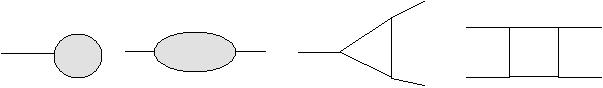
\includegraphics[width=0.5\linewidth]{master_integrals.jpg}
  \caption{Master integrals: tadpole, bubble, triangle and box}
  \label{fig-mi}
\end{figure}
Modern methods of one-loop amplitude computation are mostly based on the fact that we can decompose an amplitude in a basis with a finite number of integrals.
In massless cases, which we are most interested in, the tadpole integral vanishes. 
As a result, we can write an amplitude $A$ as
\begin{equation}\label{master_equation}
A = \sum_i c_i I_i + \mathrm{rational} + \mathcal{O}(\epsilon)
\end{equation}
where the $I_i$'s are box, triangle and bubble integrals and there may be finite polynomial term in kinematic invariants at the order of $\mathcal{O}(\epsilon^0)$
Let us follow the review done in~\cite{Gluza:2010ws} on such a basis.
\\\\
We consider integrals in $D= 4-2\epsilon$ dimension and keep external momenta to be four-dimensional.
A generic one-loop-integral can be written as
\begin{equation}\label{generic_loop_int}
I_n[P(l)] = 
-i\int\frac{\dd^D l}{(2\pi)^D}\frac{P(l)}{l^2(l-K_1)^2(l-K_{12})^2\ldots(l-K_{1\ldots (n-1)})^2}
\end{equation}
where $P$ is a polynomial in $l$.
Let us begin with integrals with high multiplicity, with five or more external legs.
In this case, we can use the Gram determinant defined as
\begin{equation}
\begin{split}
& G\begin{pmatrix}
p_1,\ldots, p_l \\
q_1,\ldots, q_l 
\end{pmatrix}
:= \det(2p_i\cdot q_j)
\\
& G(p_1, \ldots , p_l) := G\begin{pmatrix}
p_1,\ldots, p_l \\
p_1,\ldots, p_l 
\end{pmatrix}
\end{split}
\end{equation} 
to reduce the integral.
In fact, the Gram determinant vanishes if either $\{p_i\}$ or $\{q_i\}$ are linearly dependent.
One can expand each of the four-vectors $v^\mu$ in a basis of four chosen external momenta (\ie , the $K_i$'s in~\cref{generic_loop_int}) $\{b_i\}_{i=1\ldots 4}$ with the help of Gram determinants.
At one-loop, the terms $l\cdot b_i$ are reducible since we can write them as differences between terms appearing in the denominator of~\cref{generic_loop_int}.
They will lead to a sum of integrals with fewer propagators or fewer powers in $l$. 
In other words, 
\begin{equation}
I_n[(l\cdot v)^n] \rightarrow I_{n-1}[(l\cdot v)^{n-1}]\oplus I_n[(l\cdot v)^{n-1}]
\end{equation}
To prove our statement, we have to compute the contribution of five- or higher-point integrals with trivial numerator. 
We will show that they are of the order $\mathcal{O}(\epsilon)$.
Let us first consider the reduction of six- or higher-point integrals, which can be done to all orders in $\epsilon$. 
\\\\
Since the external momenta are taken in four-dimensional,
we can write the following equation involving the Gram determinant for the loop momentum $l$ and five other external momenta (denoted only by numbers) 
\begin{equation}
G\begin{pmatrix}
l & 1 & 2 & 3 & 4\\
5 & 1 & 2 & 3 & 4 
\end{pmatrix}
 = 0
\end{equation}
Accordingly, by~\cref{generic_loop_int}
\begin{equation}\label{gram_induction}
I_n\Big[G\begin{pmatrix}
l & 1 & 2 & 3 & 4\\
5 & 1 & 2 & 3 & 4 
\end{pmatrix}\Big]
 = 0
 \quad\mathrm{for}\quad n\geq 6
\end{equation}
We can expand the Gram determinant appearing in~\cref{gram_induction} into a linear combination of Gram determinants of lower order (two arrays of four vectors instead of five).
The coefficients appearing in this expansion are either of the form $(l-K_i)^2$ or $K_i$, the external momenta.
\color{red} Maybe put the expression in an Appendix ?\color{black}
As a result,~\cref{gram_induction} will give us a relationship between an $n$-point integral and $(n-1)$-point integrals.
\\\\
As for the five-point scalar integral, there might be a worry about the $\mathcal{O}(\epsilon^0)$ term or even the divergent terms.
However, divergences appear only when the loop momentum $l$ is soft or collinear to one of the external momenta according to~\cref{generic_loop_int}, where the five-point Gram determinant also vanishes. 
We conclude that
\begin{equation}
I_5[G(l,1,2,3,4)] = \mathcal{O}(\epsilon)
\end{equation}
Hence, the five-point integral can also be reduced by expanding the Gram determinant into the lower order ones.
The reduction of five- or higher-point integrals are given explicitly in~\cite{Gluza:2010ws}.
%
%






\section{Spinor-helicity formalism and color-ordered amplitudes}\label{sect-spinor}
The spinor-helicity formalism is widely used in amplitude literatures. 
One can refer to~\cite{Dixon:1996wi,Elvang:2013cua} for good introductions\footnote{The convention may change according to the signature}.
We present some useful properties under the convention used in QCD~\cite{Dixon:1996wi}.
\\\\
From a physical point of view, ampitudes should depend only on Lorentz invariant quantities that can be formed from external momenta, \eg the square $p^2$ of a four-vector $p^\mu$.
However, in most interesting models, there are not only scalar fields but also particles which have spins. 
A more suitable representation of the Lorentz group is the two-dimensional spinor representation.
We can trade a four-dimensional vector for a pair of spinors.
To be more explicit, let us consider two spinors $\bar{u}(p)$ and $v(p)$ for an outgoing massless fermion and an outgoing massless anti-fermion of momentum $p$.
They satisfy the Dirac equation and we can decompose them into two parts of different helicity:
\begin{equation}
\begin{split}
& v_+(p) = \begin{pmatrix}
|p]_\alpha \\ 0
\end{pmatrix} := \lambda_p^\alpha
\quad,\quad
v_-(p) = \begin{pmatrix}
0 \\ |p\rangle^{\dot{\alpha}}
\end{pmatrix} := \tilde{\lambda}_p^{\dot{\alpha}}
\\
& \bar{u}_-(p) = \begin{pmatrix} 
0, & \langle p |_{\dot{\alpha}})\end{pmatrix}
\quad,\quad
\bar{u}_+(p) = \begin{pmatrix} [ p|^\alpha, & 0 \end{pmatrix}
\end{split}
\end{equation} 
where $v_\pm = \frac{1}{2}(1\pm\gamma_5)v(p)$ (analog for the others) and $\alpha = 1,2$.
One should note that $u$ and $v$ are four-dimensional spinors whereas $|p\rangle$ and $|p]$ are two-dimensional objects. 
The crossing symmetry is garanteed because $v_\pm = u_\mp$.
\\
The contraction of a momentum $p$ with the gamma matrices gives
\begin{equation}\label{slashedp}
\slashed{p} = \begin{pmatrix}
0 & p_{a\dot{b}} \\ 
p^{\dot{a}b} & 0
\end{pmatrix}
\end{equation}
where 
\begin{equation}
p^{\dot{a}b} = p_\mu(\bar{\sigma^\mu})^{\dot{a}b}
\quad,\quad
p_{a\dot{b}} = p_\mu(\sigma^\mu)_{a\dot{b}}
\end{equation}
The $\sigma$'s are the Pauli matrices.
With a slight abuse of notation\footnote{
Note that $|p^\pm\rangle$ in~\cref{p_times_spinor} are two-dimensional objects, we have more precisely
\begin{equation}
\slashed{p}|p^-\rangle = p^{\dot{a}b}|p]_b
\quad,\quad
\slashed{p}|p^+\rangle = p_{a\dot{b}}|p\rangle^{\dot{b}}
\end{equation}
When multiplied with square or angle spinors, the gamma matrices are implicitly matched to the corresponding Pauli matrices.
This abuse of notation also appears in~\cref{fierz_id} and~\cref{pol_vec}.
}, the massless Dirac equation leads to
\begin{equation}\label{p_times_spinor}
\slashed{p}v_\pm (p) = \slashed{p}|p^\pm\rangle = 0
\quad \mathrm{where}\quad
|p^+\rangle := |p]
\quad,\quad
|p^-\rangle := |p\rangle
\end{equation}
The raising and lowering of spinor indices are realized by the Levi-Civita tensor
\begin{equation}\label{levi-civita}
[p|^a = \epsilon^{ab}|p] \quad,\quad
|p\rangle^{\dot{a}} = \epsilon^{\dot{a}\dot{b}}\langle p |_{\dot{b}}
\end{equation}
With the help of spinors, we can form two kinds of Lorentz invariant object
\begin{equation}\label{spinor_pdt}
\begin{split}
& \langle ij \rangle = \epsilon^{ab}(\lambda_i)_a(\lambda_j)_b = \bar{u}_-(i)u_+(j)
\\
& [ij] = \epsilon^{\dot{a}\dot{b}}(\tilde{\lambda}_i)_{\dot{a}}(\tilde{\lambda}_j)_{\dot{b}} = \bar{u}_+(i)u_-(j)
\end{split}
\end{equation}
In this formalism, the momentum can also be chosen complex. 
In the case where the momentum is real, we note from~\cref{slashedp} the relationship between the complex conjugate and the transpose of $\slashed{p}$
\begin{equation}
(\slashed{p})^* = {}^t\slashed{p}
\end{equation}
The transposition corresponds to an exchange of the square and the angle spinors. 
In other words, the chirality flip of all spinors in a spinor product is simply the complex conjugate of the spinor product
\begin{equation}
[ij] = \langle ij \rangle^* \quad\textrm{when both momenta are real with positive energies}
\end{equation}
By~\cref{levi-civita}, the spinor products defined in~\cref{spinor_pdt} are antisymmetric and the product of an angle and an square spinors vanishes. 
With this remark and a slight abuse of notation, one has, from the completeness relation of spinors,
\begin{equation}\label{p_splinors}
\slashed{p} = |p\rangle [p| + |p]\langle p|
\end{equation}
For computational purpose, we give here two useful identities
\begin{enumerate}
\item \textbf{Fierz' identity} 
\begin{equation}\label{fierz_id}
\langle 1 |\gamma^\mu |2]\langle 3 |\gamma^\mu|4] = 2\langle 13 \rangle [42]
\end{equation}
\item \textbf{Schouten's identity} 
\begin{equation}
\langle ij \rangle \langle lk \rangle + \langle ik\rangle \langle jl\rangle + \langle il \rangle \langle kj \rangle = 0
\end{equation}
\end{enumerate}
where $|i^\rangle$ stands for the angle spinor for the particle having momentum $p_i$ (analogously for the square spinor). 
These identities can be easily shown.
For the first one, the properties of the Pauli matrices are used.
The second one can be derived from the fact that the spinors used here are two-dimensional objects, so a spinor can always be written as linear combination of two other independent ones.
%
\\\\
In presence of massless vectors, we can write the corresponding polarization vectors by choosing an arbitrary reference momentum $q$ which is not collinear to the momentum $p$ of the vector field:
\begin{equation}\label{pol_vec}
\begin{split}
& \varepsilon^+_\mu (p, q) = \frac{\langle q | \gamma_\mu |p]}{\sqrt{2}\langle qp \rangle}
\\
& \varepsilon^-_\mu (p, q) = -\frac{[q|\gamma_\mu | p\rangle}{\sqrt{2}[qp]}
\end{split}
\end{equation}
One can check that these polarization vectors are transverse and give us the expected results from Feynman diagram computations. 
%
%
\subsection*{Color-ordered amplitudes}
In a Yang-Mills theory, the vertices become color-dependent. 
However, in some specific cases, it is possible to separate into 
a color-dependent part and a kinematic-dependent partial amplitude using the property of the structure constant.
To be more precise, an all-gluon QCD $n$-point amplitude at tree-level can be decomposed into~\cite{MANGANO1988461}
\begin{equation}\label{color-ordered}
\mathcal{A}_n^{\mathrm{tree}}(g_1, \ldots, g_n) = g'^{n-2}\sum_{\sigma\in\textrm{ permutation of }\{2,\ldots\}} A_n[1,\sigma(2),\ldots,\sigma(n))]\tr(T^{a_1} T^{a_{\sigma(2)}}\ldots T^{a_{\sigma(n)}})
\end{equation}
where $g'$ is the coupling constant, the $T^{a_i}$'s are generators of the gauge group and the $A_n[\ldots]$'s are the partial amplitudes.
Partial amplitudes are called color-ordered amplitudes because the color configuaration determines the order of the species appearing in the argument.
As one notices from the definition~\cref{color-ordered}, the cyclicity of the trace implies that color-ordered amplitudes are also cyclic. 
In this report, we will essentially give examples of all-gluon amplitudes.
As we are going to see, color-ordered all-gluon amplitudes have some nice and compact expressions.
\color{red} say something about one-loop\color{black}
%
%
\subsection*{3-point kinematics}
The first non-trivial objects to compute at tree-level are three-point amplitudes $A_3[1^{h_1}2^{h_2}3^{h_3}]$, where the $h_i$'s denote the helicities.
We can compute them directly by applying Feynman rules. 
We list here the only two non-vanishing three-point gluon amplitudes (the coupling constant is omitted)
\begin{equation}
\begin{split}
& A^{\mathrm{tree}}_3[g_1^- g_2^- g_3^+] = \frac{\langle 12 \rangle^3}{\langle 13 \rangle \langle 32 \rangle}
\\
& A^{\mathrm{tree}}_3[g_1^+ g_2^+ g_3^-] = \frac{ [12]^3}{[13 ][ 32 ]}
\end{split}
\end{equation}
Meanwhile, their forms may be guessed even before explicit calculations.  
By momentum conservation, we have $p_3^2 = (p_1 + p_2)^2 = \langle 12\rangle[21] = 0$. 
If we allow complex momenta, the spinor products can be non simultaneously vanishing (since they are not related by complex conjugation any more). 
As a result, either the square or the angle product vanishes.
Thus, a 3-point amplitude contains only square products or angle products. 
Let us take the example of $A_3[1^{-}2^{-}3^{+}]$.
We may write an ansatz for it\footnote{One might construct an ansatz with only square products. However, it should be discarded because it will not give the right dimension.} :
\begin{equation}
A_3[1^{-}2^{-}3^{+}] = c\langle 12 \rangle^{x_{12}}\langle 23 \rangle^{x_{23}}\langle 31 \rangle^{x_{31}}
\end{equation}
\cref{p_splinors} implies that the momentum $p$ remains invariant under the following transformations, called \textbf{little group scaling}\footnote{This rule is valid for spin-0, $\frac{1}{2}$ and 1 particles. 
For spin-0 ones, the validity of the relation is clear because scalar fields do not scale with the little group scaling.
Whereas for spin-1 particles, one can verify the relationship by looking at how polarization vectors scale under the little group scaling.
}
\begin{equation}
|p\rangle \rightarrow t| p\rangle \quad,\quad 
|p]\rightarrow t^{-1} |p]
\end{equation} 
A consequence of this is the scaling rule for amplitudes while an external leg is rescaled
\begin{equation}
A_n \big(\{ |1\rangle, |1], h_1\},\ldots,\{t_i|i\rangle, t_i^{-1}|i], h_i\},\ldots\big) = 
t_i^{-2h_i}A_n(\ldots, \{|i\rangle,|i], h_i\},\ldots)
\end{equation}
Therefore, in the case of all-gluon, we have
\begin{equation}
A_3[g_1^-g_2^-g_3^+] = c\frac{\langle 12\rangle^3}{\langle 23 \rangle\langle 31\rangle}
\end{equation}
This corresponds to the answer obtained from direct computations.
%
%
\subsection*{Maximally-helicity-violating amplitudes and the Taylor-Parke formulae for gluons}
Consider now $n$-point all-gluon amplitudes for $n\geq 4$. 
By well choosing the reference momenta for the polarization vectors, we can show (see p.31 of~\cite{Elvang:2013cua}) that the following all-gluon amplitudes vanishes at tree-level
\begin{equation}
A_n[g_1^\pm \ldots g_n^\pm] = A^{\mathrm{tree}}_n[g_1^\pm \ldots g_i^\mp \ldots g_n^\pm] = 0
\end{equation}
for $n\geq 4$.
In other words, when all the external legs have the same helicity or only one is different from the others, the tree-level amplitude vanishes.
The first class of non-vanishing tree amplitudes is the \textbf{maximally-helicity-violating (MHV)} amplitudes.
These are amplitudes which break maximally the helicity conservation, having exactly two external legs have helicity different from the rest.
The MHV gluon amplitudes can be written in a surprisingly simple form
\begin{equation}
\begin{split}
& A_n[1^+\ldots i^-\ldots j^-\ldots n^+] = 
\frac{\langle ij \rangle^4}{\langle 12 \rangle\ldots \langle n1 \rangle}
\\
& A_n[1^-\ldots i^+\ldots j^+\ldots n^-] = 
\frac{[ ij]^4}{[ 12 ]\ldots [n1 ]}
\end{split}
\end{equation}
These are called the \textbf{Parke-Taylor formulae}, first conjectured in~\cite{PhysRevLett.56.2459} and later proven by Berends and Giele by using the off-shell recursion~\cite{BERENDS1988759}. 
A more recent approach to prove these formulae is the BCFW on-shell recursion~\cite{BRITTO2005499, PhysRevLett.94.181602}, which will be presented in the next section. 







%\section{Triple cut, triangle and bubble coefficients in $D=4$}\label{sect-triple_cut}
We are now left with triangle and bubble coefficients to determine. 
Forde proposed a method using triple cut to determine the triangle and bubble coefficients in one-loop in four-dimension~\cite{Forde:2007mi}.
This method consists in choosing a good parametrization for the loop momentum after applying cuts such that the triangle and bubble contributions can be distiguished from the box contributions.
In this method, we consider four dimensional loop momentum.
\begin{figure}[h]
  \centering
  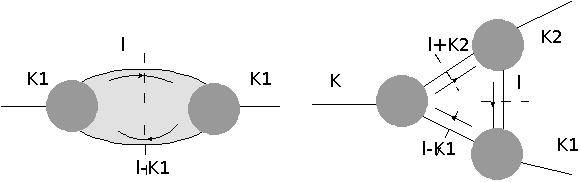
\includegraphics[width=0.8\linewidth]{triple_cut.jpg}
  \caption{The two particle cut and triple cut used in this section}
  \label{fig-triple_cut}
\end{figure}
%
\subsection*{Triangle coefficient} 
Upon applying a triple cut, the three delta functions leave only one degree of freedom in four-dimension. 
Let us denote it by $t$.
The most general expression for a cut amplitude takes the form 
\begin{equation}\label{tricut}
(2\pi)^3\int\dd l^4 \prod_{i=0}^2 \delta(l_i^2) A_1A_2A_3 = 
(2\pi)^3\int\dd l^4 \prod_{i=0}^2 \delta(l_i^2)\Big(\mathrm{Inf}_t(A_1A_2A_3)(t) + \sum_{\textrm{$t_j$ poles}}\frac{\res_{t = t_j}A_1 A_2 A_3}{t-t_j}\Big)
\end{equation}
where the $A$'s are tree amplitudes and the first term on the right-hand side is a polynomial in $t$ defined by
\begin{equation*}
\lim_{t\rightarrow\infty}\big([\mathrm{Inf}_tA_1A_2A_3](t) - A_1A_2A_3(t)\big) = 0
\end{equation*}
In most of cases, the propagators of the type $\frac{1}{(l-P)^2}$ contain two poles that can be expressed in terms of $t$. 
The second part of~\cref{tricut} can hence be considered as contributions of cut boxes. 
As a result, the information on the bubble and triangle contributions is only contained in the first term on the \rhs of~\cref{tricut}.
According to Forde, we can choose a parametrization such that only the constant term in the polynomial $\mathrm{Inf}_t(A_1A_2A_3)(t)$ contributes to the integral. 
%
\\\\
Consider a triple cut leading to the constraints\footnote{Here we take $-K_2$ instead of $K_2$ in the triangle diagram of figure~\ref{tricut}, which is the choice used in Forde's original paper.}
\begin{equation*}
l^2 = (l-K_1)^2 = (l - K_2)^2 = 0
\end{equation*}
One can construct two null vectors $K_1^\flat$ and $K_2^\flat$ from the external momenta $K_1$ and $K_2$ 
\begin{equation}\label{k_flat}
K_1^\flat = K_1 - \frac{S_1}{\gamma}K_2^\flat \quad\quad
K_2^\flat = K_2 - \frac{S_2}{\gamma}K_1^\flat
\end{equation}
%
where $S_i = K_i^2$ and $\gamma = \langle K_1^\flat|K_2^\flat|K_1^\flat] =\langle K_2^\flat|K_1^\flat|K_2^\flat]$.
There are two possibilities for $\gamma$
\begin{equation}\label{sol_for_gamma}
\gamma_{\pm} = (K_1\cdot K_2) \pm\sqrt{\Delta}\quad
\mathrm{where}\quad
\Delta = (K_1\cdot K_2)^2 - K_1^2K_2^2
\end{equation}
In terms of the spinor components, the constraints require
\begin{equation}\label{l_param}
\langle l | = t\langle K_1^\flat| + \alpha_{01}\langle K_2^\flat| \quad\quad
[ l | = \frac{\alpha_{02}}{t}[ K_1^\flat| + [ K_2^\flat|
\end{equation}
where
\begin{equation*}
\alpha_{01} = \frac{S_1(\gamma S_2)}{\gamma^2 - S_1S_2}\quad \quad
\alpha_{02} = \frac{S_2(\gamma S_1)}{\gamma^2 - S_1S_2}
\end{equation*}
%
and, as a four-vector,
\begin{equation*}
l^\mu = \alpha_{02} K_1^{\flat,\mu} + \alpha_{01}K_2^{\flat,\mu} + \frac{t}{2}\langle K_1^\flat | \gamma^\mu |K_2^\flat] + \frac{\alpha_{01}\alpha_{02}}{2t}\langle K_2^\flat|\gamma^\mu |K_1^\flat]
\end{equation*}
%
Now, we can use an argument similar to the one in~\cite{Ossola:2006us} on the spurious term to find the vanishing integrals.
\color{red}Appendix ?\color{black}
%
%%%%%%%%%%%%% not used
\iffalse
To illustrate this argument, we consider the case of a rank-1 3-point-like integral. 
By simple arguments on the rank and the dependence on external momenta, 
\begin{equation*}
\int\dd^D q \frac{q^\mu}{D_0(q)D_1(q+p_1)D_2(q+p_2)} = c_1p_1^\mu + c_2p_2^\mu
\end{equation*}
If we contract the above relation with a vector $v^\mu$ orthogonal to $p_1$ and $p_2$, we obtain a vanishing integral.
$q\cdot v$ is hence a spurious term.
The same technique can be applied to show that $(q\cdot v)^n$ is spurious for any $n>0$. 
\fi
%%%%%%%%%%%%%%%%%%%5 end of not used
%
We can use the fact that $\langle K_1^{\flat,\pm} | K_{1,2}|K_2^{\flat,\pm}\rangle = 0 $ and $\langle K_1^{\flat,\pm}|\gamma^\mu|K_{2}^{\flat,\pm}\rangle\langle K_1^{\flat,\pm}|\gamma_\mu|K_{2}^{\flat,\pm}\rangle = 0$
to show that all only the constant term in the polynomial $\mathrm{Inf}_t(A_1A_2A_3)(t)$ contributes to~\cref{tricut}. 
The other two loop-momenta, $l_1 = l-K_1$ and $l_2 = l-K_2$, are parametrize in a similar way in~\cref{l_param} by replacing $\alpha_{01}$ and $\alpha_{i2}$ by $\alpha_{i1}$ and $\alpha_{i2}$ given in~\cite{Forde:2007mi}.
%
%
\subsection*{Two-particle cuts and scalar bubble coefficients}
Triple cuts can also be used to determine bubble coefficients. 
Let us first consider a two-particle cut (cf. figure~\ref{fig-triple_cut}).
Contrary to the previous case, we will have two free parameters $y$ and $t$.
\begin{equation}\label{2-part_cut}
\begin{split}
(2\pi)^2\int \dd^4 l \prod_{i=0}^1 \delta(l_i^2) A_1 A_2 = & 
(2\pi)^2\int \dd t\dd y J_{t,y}\Big(\big[\mathrm{Inf}_t [\mathrm{Inf}_y(A_1A_2)](y)\big](t) 
\\&
+
\mathrm{Inf}_t\big(\sum_{\textrm{poles}}\frac{\mathrm{Res}_{y = y_i}A_1A_2}{y-y_j})
+
\mathrm{Inf}_t\big(\sum_{\textrm{poles}}\frac{\mathrm{Res}_{t = t_l}\mathrm{Inf}_y A_1A_2}{t-t_l})
\\ &
+
\mathrm{Inf}_t\big(\sum_{\textrm{poles}}\frac{\mathrm{Inf}_t\big(\sum_{\textrm{poles}}\frac{\mathrm{Res}_{y = y_i}A_1A_2}{y-y_j}\big)}{t-t_l}\big)
\Big)
\end{split}
\end{equation}
We parametrize the loop momentum $l$ by
\begin{equation*}
l^\mu = yK_1^{\flat,\mu} + \frac{S_1}{\gamma}(1-y)\chi^\mu + \frac{t}{2}\langle K_1^\flat|\gamma^\mu|\chi] + \frac{S_1}{2\gamma}\frac{y}{t}(1-y)\langle \chi|\gamma^\mu|K_1^\flat]
\end{equation*}
where
\begin{equation*}
K_1^\flat = K_1 - \frac{S_1}{\gamma}\chi^\mu ,\quad
\gamma = \langle \chi | \slashed{K}_1^\flat|\chi]
\end{equation*}
and $\chi$ is an arbitrary null vector (non-collinear to $K_1$).
\\
As in the triangle case, we can use $\langle K_1^\flat| \slashed{K}_1|\chi] = \langle K_1^\flat|\slashed{K}_1 | \gamma^\mu|\chi]\langle K_1^\flat|\gamma_\mu|\chi]= 0$ to show that
\begin{equation*}
\int\dd t\dd y J_{t,y}t^n = \int \dd t \dd y \big(\frac{y}{t}\big)^n(1-y)^n = 0
\quad\Rightarrow\quad
\int \dd t \dd y J_{t,y}t^n = 0
\quad\textrm{for}\quad n\neq 0
\end{equation*} 
From the Passarino-Veltman reduction, we are able to conclude that all integrands of the type $t^0y^m$ are non-vanishing, which makes difference \wrt the triple cut case. 
Naively, one might think that the bubble coefficients come from the first term of~\cref{2-part_cut}.
However, the loop momentum parametrization that has been used leads to more non-vanishing terms than in the triple cut case. 
Furthermore, the second and the third terms in~\cref{2-part_cut} can be reduced to scalar bubble integrals plus triangle integrals. 
In order to relate the contribution to the bubble coefficient of the residue piece, we apply an additional constraint: $(l+K_2)^2=0$ to the two-particle cut.
This will then fix the free parameter $y$.
The integral will then take the form
\begin{equation*}
(2\pi)^3\int \dd t \dd y J_t'\big(\delta(y-y_+) + \delta(y-y_-)\big) \mathcal{M}(y,t) = -2(2\pi)^2 i \int \dd t \dd y J_{t,y}\mathrm{Res}_{y = y_{\pm}}\frac{\mathcal{M}(y,t)}{(l+K_2)^2}
\end{equation*}
where $\mathcal{M}(y,t)$ is a general cut integral and $J_t'$ a function of $t$.
Therefore, the residue contributions are, up to a factor of $-\frac{1}{2}$, given by the triple cut.
As discussed in the previous subsection, the $t^0$ contribution in the triple cut gives the triangle coefficients ant the other terms in power of $t$ give the scalar bubble coefficients.
\\\\
We will just list here the final result without giving computational details which involve calculations of non-vanishing integrals and reduction techniques.
The bubble coefficient is given by
\begin{equation*}
b = -i[\Inf_t[\Inf_y A_1 A_2](y)](t)\big|_{t\rightarrow 0 , y^m\rightarrow \frac{1}{m+1}}
-\frac{1}{2}\sum_{C_{\mathrm{tri}}}[\Inf_t A_1A_2A_3](t)\big|_{t^j\rightarrow T(j)}
\end{equation*}
where the subscripts indicate the substitutions to be done and $T(j)$ is given in eq.(5.26) of~\cite{Forde:2007mi}. 
The second term above is summed over all possible triangle configurations.
\\\\
%%%%%% not used
\iffalse
As an example, let us cite briefly how the two-mass linear triangle
\begin{equation*}
(2\pi)^2\int\dd^4 l \prod_{i=0}^1\delta(l_i^2)\frac{\langle K_2|\slashed{l}|K_1]}{(l+K_2)^2}
\end{equation*}
is treated in~\cite{Forde:2007mi}:
\begin{enumerate}
\item Do a two-particle cut. We will then get two terms in the integrand: one in $y^0$ and a residual term. The term in $y^0$ gives us a contribution to the bubble coefficients; while the residual term means that a triple cut is needed to get the contributions to the bubble and triangle contributions.
%
\item Apply a triple cut. There will be a term in $t$ if we choose the parametrization introduced previously, which encodes information on the bubble coefficients.
%
\item This term then requires the knowledge of $\int \dd t J_t' t$, which can be re-expressed in terms of our parametrization. Then, apply the Passarino-Veltman reduction to get the relationsship between $\int \dd tJ_t' t$ and the cut bubble $B_0^{\mathrm{cut}(K_1^2)}$
\end{enumerate}
\fi
% end of not used
%
%
%
\subsection{Example: triangle coefficient extraction for six-photon amplitude in QED}
Let us show explicitly how to extract the coefficient for scalar triangle using the example of the six-photon amplitude $A_6[1^-2^+3^-4^+5^-6^+]$ in QED.
This example is given in~\cite{Forde:2007mi}.
\begin{figure}
  \centering
  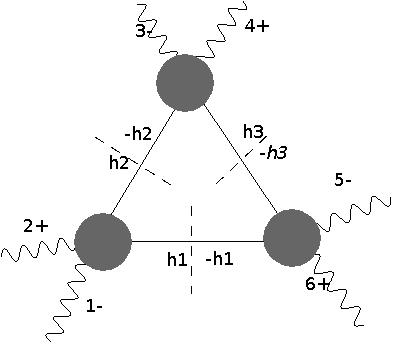
\includegraphics[width=0.5\linewidth]{6photons.jpg}
  \caption{Triple cut for the six-photon example}
  \label{fig-6photons}
\end{figure}
First, we have to compute the tree-level four-point amplitude $A_4[1^{h_1}2^{h_2}3^{h_3}4^{h_4}]$. 
Contrary to non-abelian theories, the four-photon amplitude vanishes at tree-level in QED.
Thus, the relevant four-point amplitudes are following ones which containt two photons and two fermions
\begin{equation*}
A_4^{\mathrm{tree}}(\bar{f}_1^- f_2^+ \gamma_1^-\gamma_2^+)
\quad,\quad
A_4^{\mathrm{tree}}(\bar{f}_1^+ f_2^- \gamma_1^-\gamma_2^+)
\end{equation*}
Recall that the polarization vectors contracted with the $\gamma$-matrices are represented by\footnote{This can be shown using the expression given previously and the Fierz identity.}
\begin{equation*}
\begin{split}
& \slashed{\epsilon}_+(p,k) = -\frac{\sqrt{2}}{\langle kp\rangle}\big(|p]\langle k| + |k\rangle[p|\big)
\\
& \slashed{\epsilon}_-(p,k) = \frac{\sqrt{2}}{[kp]}\big(|p\rangle [k| + |k]\langle p|\big)
\end{split}
\end{equation*}
We denote the out-going fermion momenta by $q_i$ and the out-going photon momenta by $p_i$. 
A direct Feynman diagram computation gives\footnote{Recall that we take all the particles out-going in our convention.}
\begin{figure}[h]
  \centering
  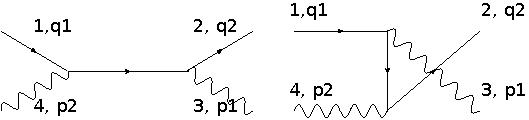
\includegraphics[width=0.8\linewidth]{qed.jpg}
  \caption{$s$-channel (left) and $u$-channel (right)}
  \label{fig-qed}
\end{figure}
%
\begin{equation*}
\begin{split}
A_{4}^{\mathrm{tree}}(\bar{f}_1^- f_2^+ \gamma_1^-\gamma_2^+) 
= &
\frac{ie^2}{(-p_1 - q_1)^2}\langle q_1, p_1\rangle \frac{\sqrt{2}}{[k, p_1]}
[k|\big(|p_2] \langle p_2| + |q_2]\langle q_2|\big)
\frac{\sqrt{2}}{\langle k p_2\rangle}
\big(|p_2]\langle k| + |k\rangle[p_2|\big) |q_2]
\\
&
+\frac{ie^2}{(-q_1-p_2)^2}\langle q_1, k'\rangle
\frac{\sqrt{2}}{\langle k', p_2\rangle}[p_2|
\big( -|p_2]\langle p_2| - |q_1]\langle q_1|\big)
\frac{\sqrt{2}}{[k', p_1]}|k'\rangle [p_1, q_2]
\end{split}
\end{equation*}
The first term corresponds to the $u$-channel (cf. figure~\ref{fig-qed}) and the second one $s$-channel.
By choosing the reference momentum $k'$ to be $q_1$, the second term above vanishes. 
We can choose $k = q_2$ and get 
\begin{equation}\label{4pt_qed1}
\begin{split}
A_{4}^{\mathrm{tree}}(\bar{f}_1^- f_2^+ \gamma_1^-\gamma_2^+) 
= &
\frac{2ie^2\langle q_1 p_1 \rangle[p_2 q_2]^2}{[q_2 p_1](p_1+q_1)^2}
\\ 
= &
\frac{2ie^2[42]^2}{[23][31]}
\end{split}
\end{equation}
where in the last equation, the particles are indexed in the order in which they appear in the argument of the amplitude.
In the same manner, there is an $u$-channel and an $s$-channel contribution for the other relevant four-point amplitude. 
The $u$-channel can be made vanishing by choosing properly the reference momentum. 
If we choose the reference momentum for the $s$-channel to be $q_2$, we find 
\begin{equation}\label{4pt_qed2}
A_4^{\mathrm{tree}}(\bar{f}_1^+ f_2^- \gamma_1^- \gamma_2^+) = 
\frac{2ie^2\langle 32\rangle^2}{\langle 41 \rangle\langle 24\rangle}
\end{equation}
Applying a triple cut on the channel $12:34:56$ (cf. figure~\ref{fig-6photons}), we get the two contributing cut amplitudes
\begin{equation}\label{triple_cut_1}
A_{4}^{\mathrm{tree}}(f_1^- 1^-2^+\bar{f}_3^+)
A_4^{\mathrm{tree}}(\bar{f}_1^+f_2^-5^-6^+)
A_4^{\mathrm{tree}}(\bar{f}_2^+ f_3^-3^-4^+)
=
-8ie^6\frac{\langle l_1 1\rangle^2 \langle 5l_2 \rangle^2\langle 3l_3\rangle^2}{\langle2 l_3\rangle\langle l_1 2\rangle\langle 6 l_1 \rangle\langle l_2 6\rangle\langle 4 l_2\rangle\langle l_3 4\rangle}
\end{equation}
\begin{equation}\label{triple_cut_2}
A_{4}^{\mathrm{tree}}(f_1^+ 1^-2^+\bar{f}_3^-)
A_4^{\mathrm{tree}}(\bar{f}_1^-f_2^+5^-6^+)
A_4^{\mathrm{tree}}(\bar{f}_2^- f_3^+3^-4^+)
=
-8ie^6\frac{[2l_1]^2[6l_2]^2[4l_3]^2}{[l_1 1 ][1l_3][l_2 5][5l_1][l_2 3][3l_3]}
\end{equation}
where $l_i$ stands for momentum of the outgoing fermion $f_i$.
Under the triple cut parametrization,~\cref{triple_cut_1} and~\cref{triple_cut_2} lead to the same contribution. 
In fact, the ratio of~\cref{4pt_qed1} to~\cref{4pt_qed2} gives
\begin{equation*}
\frac{[42]^2}{[23][31]}\frac{\langle 41\rangle\langle 24\rangle}{\langle 32 \rangle^2} = \frac{\langle 31\rangle[42]}{\langle 32 \rangle[41]} 
\end{equation*} 
Hence the ratio of~\cref{triple_cut_1} to~\cref{triple_cut_2} is
\begin{equation*}
\frac{[4l_2]\langle 3l_3\rangle}{[4l_3]\langle 3l_2\rangle}
\frac{[6l_1]\langle 5l_2\rangle}{[6l_2]\langle 5l_1\rangle}
\frac{[2l_3]\langle 1l_1\rangle}{[2l_1]\langle 1l_3\rangle}
\end{equation*}
Since the contribution to triangle coefficient is given by taking the $\Inf$ of~\cref{triple_cut_1} and~\cref{triple_cut_2}, we are interested in the $\Inf$ part of the above under the parametrization~\cref{l_param}, which gives
\begin{equation*}
\Inf\Big(\frac{([4K_2^\flat] + \frac{\alpha_{12}}{t}[4K_1^\flat])(t\langle 3K_1^\flat \rangle + \alpha_{21}\langle 3K_2^\flat\rangle)}{([4K_2^\flat] + \frac{\alpha_{22}}{t}[4K_1^\flat])(t\langle 3K_1^\flat \rangle + \alpha_{11}\langle 3K_2^\flat\rangle)}(\ldots)\Big)
= 1
\end{equation*} 
%
Thus, the total contribution is twice of~\ref{triple_cut_1}, or in a more explicit form using~\cref{l_param}\footnote{
Note that here we apply an offset of one to the indices \wrt the previous notation.
}
\begin{equation*}
\begin{split}
-32ie^6 & \frac{(t\langle K_1^\flat 1 \rangle + \alpha_{01}\langle K_2^\flat 1\rangle)^2
(t\langle K_1^\flat 5 \rangle + \alpha_{11}\langle K_2^\flat 5\rangle)^2
(t\langle K_1^\flat 3 \rangle + \alpha_{21}\langle K_2^\flat 3\rangle)^2
}{
(t\langle 2K_1^\flat  \rangle + \alpha_{21}\langle 2 K_2^\flat \rangle)
(t\langle K_1^\flat 2 \rangle + \alpha_{01}\langle K_2^\flat 2\rangle)
(\langle  6K_1^\flat  \rangle + \alpha_{01}\langle  6K_2^\flat \rangle)^2
(t\langle K_1^\flat 6 \rangle + \alpha_{11}\langle K_2^\flat 6\rangle)}
\\
&\times
\frac{1}{
(t\langle 4K_1^\flat  \rangle + \alpha_{11}\langle 4 K_2^\flat \rangle)
(t\langle K_1^\flat 4 \rangle + \alpha_{21}\langle K_2^\flat 4 \rangle)
}
\end{split}
\end{equation*}
As a last step, we obtain the triangle coefficient by taking the $\Inf$ of the above and average over all possible solution for the $\gamma_\pm$~\cref{sol_for_gamma}
\begin{equation*}
16ie^6\sum_{\gamma_\pm}\frac{\langle K_1^\flat 1 \rangle^2\langle K_1^\flat 5\rangle^5 \langle K_1^\flat 3 \rangle^2}{\langle K_1^\flat 2 \rangle^2\langle K_1^\flat 6\rangle^2 \langle K_1^\flat 4 \rangle^2}
\end{equation*}
Substituting $K_1^\flat$ by its expression~\cref{k_flat}, we obtain an agreement with~\cite{Forde:2007mi}.











%\section{Forumlae}

\paragraph{Beta function}
\begin{equation*}
B(a,b) = \int_0^1 \dd x (1-x)^{a-1}x^{b-1} = \frac{\Gamma(a)\Gamma(b)}{\Gamma(a+b)}
\end{equation*}

\paragraph{Hypergeometric function}
\begin{equation*}
_2F_1(a,b,c;z) = \frac{\Gamma(c)}{\Gamma(b)\Gamma(c-b)}\int_0^1\frac{t^{b-1} (1-t)^{c-b-1}}{(1-tz)^a} \dd t
\end{equation*}
%
\begin{equation*}
\begin{split}
_2F_1(a,b,c;z) & = (1-z)^{-a}(_2F_1)(a,c-b,c;\frac{z}{z-1})
\\
& = (1-z)^{-b}(_2F_1)(c-a,b,c;\frac{z}{z-1})
\\
& = (1-z)^{c-a-b}(_2F_1)(c-a,c-b,c;z)
\end{split}
\end{equation*}
%
\begin{equation*}
_2F_1(a,b,c;z) = 1 + \frac{ab}{1!c} + \frac{a(a+1)b(b+1)}{2!c(c+1)}z^2 + \ldots
=\sum_{n=0}^{\infty}\frac{(a)_n(b)_n}{(c)_n}\frac{z^n}{n!}
\end{equation*}


\paragraph{$D$-dimensional sphere ($(D-1)$-sphere) measure }
\begin{equation*}
\int \dd \Omega_{D} = \int^\pi_0 \dd \theta_{D-1}\sin^{D-2} \theta_{D-1} \times \ldots \times \int^\pi_0 \dd \theta_2 \sin\theta_2 \int^{2\pi}_0 \dd \theta_1
\end{equation*}

\begin{equation*}
\Omega_D = \int \dd \Omega_D = \frac{2\pi^{D/2}}{\Gamma(\frac{D}{2})}
\end{equation*}
%wrong....different notations
%\begin{equation*}
%\int\dd \Omega_{D+1} = 2\pi^{D-2}\frac{1}{\Gamma(\frac{1}{2}D)}\int^{\pi}_0\dd \theta_D \sin^{D-1}\theta_D
%\end{equation*}

%\begin{equation*}
%\Omega_{D+1} = 2^D \pi^{D/2} \frac{\Gamma(\frac{1}{2}D)}{\Gamma(D)}
%\end{equation*}

\paragraph{Gamma function}
\begin{equation*}
\Gamma(\epsilon) = \frac{1}{\epsilon} - \gamma_E + \mathcal{O}(\epsilon)
\end{equation*}

\paragraph{Feynman parametrization}
\begin{equation*}
\frac{1}{\prod_{i=1}^n A_i} = \int_0^1 \dd x_1 \ldots\int^1_0\dd x_n\frac{(n-1)!\delta(\sum_{i=1}^n x_i -1)}{(\sum_{i=1}^n x_i A_i)^n}
\end{equation*}

\paragraph{Useful integrals}
\begin{equation*}
\int\frac{\dd^D k}{(2\pi)^D}\frac{k^{2a}}{(k^2-\Delta)^b} = i(-1)^{a-b}\frac{1}{(4\pi)^{D/2}\Delta^{b-a-D/2}}\frac{\Gamma(a+D/2)\Gamma(b-a-D/2)}{\Gamma(b)\Gamma(D/2)}
\end{equation*}


%\appendix
%\include{data/chap-appendix/appendix}

%\addcontentsline{toc}{chapter}{Bibliography} 
\bibliography{biblio}
\bibliographystyle{unsrt}

\end{document}
